% Chapter 1
\chapter{Marco Teórico} % Main chapter title

\label{Cap_SDT} % For referencing the chapter elsewhere, use \ref{Chapter1} 

%----------------------------------------------------------------------------------------

% Define some commands to keep the formatting separated from the content 
\newcommand{\keyword}[1]{\textbf{#1}}
\newcommand{\tabhead}[1]{\textbf{#1}}
\newcommand{\code}[1]{\texttt{#1}}
\newcommand{\file}[1]{\texttt{\bfseries#1}}
\newcommand{\option}[1]{\texttt{\itshape#1}}

%----------------------------------------------------------------------------------------

\section{Teoría de Detección de Señales}

%Detectar ciertos estados en el mundo es importante para guiar nuestro comportamiento
Uno de los problemas más frecuentes a los que se enfrentan los organismos como sistemas inmersos en entornos variables que buscan optimizar su comportamiento, es la detección de estados o eventos específicos (\textbf{señales}) que de acuerdo a su experiencia y tras la definición de ciertas relaciones de contingencia, les proporcionen información relevante sobre el estado del mundo, las restricciones vigentes y la disponibilidad de eventos biológicamente importantes (McNicol, \citeyear{McNicol1}).\\

%Origen y expansión de la Teoría de Detección de Señales en la psicología y otras áreas
La Teoría de Detección de Señales (SDT, por sus siglas en inglés) aparece por primera vez en 1954 -como tantos otros avances científicos y tecnológicos motivados por las necesidades planteadas por la Segunda Guerra Mundial- en el contexto del estudio y desarrollo de radares para detectar señales eléctricas específicas (Peterson, Birdsall y Fox, \citeyear{Peterson1954}). Muy poco tiempo después, los psicólogos John A. Swets y Wilson P. Tanner contribuyeron a la expansión de la teoría a un contexto psicológico, como un modelo para estudiar la percepción de los organismos (Tanner y Swets, \citeyear{Tanner1954}; Swets, Tanner y Birdsall, \citeyear{Swets1961}). Desde entonces, la SDT constituye uno de los modelos más estudiados, desarrollados y ampliamente aplicados en Psicología (Stainslaw y Todorov, \citeyear{Stainslaw1999}), extendiéndose desde su foco inicial en el estudio de la percepción (Rosenholtz, \citeyear{Rosenholtz2001}; Pessoa, Japee y Ungerleider, \citeyear{Pessoa2005}; Wallis y Horswill, \citeyear{Wallis2007}) hacia el estudio de cualquier fenómeno o escenario donde los organismos se enfrenten al problema de emitir -y guiar su comportamiento en función a- juicios de detección; por ejemplo, en materia de la emisión de diagnósticos clínicos (Grossberg y Grant, \citeyear{Grossberg1978}; Swets, Dawes y Monahan, \citeyear{Swets2000}; Boutis, Pecaric, Seeto y Pusic, \citeyear{Boutis2010}), en el estudio de ciertas condiciones clínicas (Westermann y Lincoln, \citeyear{Westermann2010}; Bonnel y cols., \citeyear{Bonnel2003}; Brown, Kosslyn, Breiter, Baer y Jenike, \citeyear{Brown1994}; Naliboff y Cohen, \citeyear{Naliboff1981}), en el estudio de la identificación visual de testigos (Gronlund, Wixted y Mickes, \citeyear{Gronlund2014}; Wixted y Mickes, \citeyear{Wixted2014}; Wixted, Miches, Dunn, Clark y Wells, \citeyear{Wixted2016}) y un muy amplio \textit{etcétera} (Gordon y Clark, \citeyear{Gordon1974}; Nuechterlein, \citeyear{Nuechterlein1983}; Harvey Jr., Hammond, Lusk y Mross, \citeyear{Harvey1992}; Verghese, \citeyear{Verghese2001}).\\ 

%La Teoría de Detección de señales como un modelo descriptivo para el problema de la detección que admite la importancia de la incertidumbre, como parte del entorno y como motor en el uso de sesgos de respuesta.
La SDT constituye un modelo estadístico que describe el problema al que se enfrentan los organismos inmersos en situaciones de detección en ambientes con incertidumbre, donde las \textit{señales} -los estímulos cuya ocurrencia interesa detectar- coexisten con \textit{ruido} -estímulos que no son la señal pero que pueden confundirse con esta-. Se trata de un modelo de decisión que entiende la detección como una tarea de elección, donde los organismos no responden simplemente con base en lo que perciben, sino que emiten el juicio de detección que les permita guiar su comportamiento de la manera mas óptima posible dada la información que poseen sobre su entorno y la evidencia presente (Swets y cols., \citeyear{Swets2000}; Killeen, \citeyear{Killeen2014}).\\

La generalizabilidad del modelo de la SDT al estudio de distintos fenómenos y tareas de detección es posible gracias a lo abstracto de sus elementos: la señal que interesa detectar puede ser desde un estímulo concreto -una luz o un tono- hasta la pertenencia a una categoría -una enfermedad o amenaza- y el ruido es simplemente todo elemento presente en el entorno de la tarea que no sea la señal (Stainslaw y Todorov, \citeyear{Stainslaw1999}; McNicol, \citeyear{McNicol1}).\\ 


\subsection{Supuestos generales del modelo}

%La TDS distingue dos grandes factores en la emisión de un juicio o respuesta: La discriminabilidad y el sesgo.
La SDT funciona como una herramienta -o marco de análisis- para traducir el desempeño observado en tareas de detección en inferencias sobre la precisión con que la señal se distingue del ruido (la \textbf{discriminabilidad}) y la posible preferencia -o tendencia- del sistema detector a responder en favor o en contra de su detección, de acuerdo a la estructura de la tarea y las consecuencias comprometidas (el \textbf{sesgo}), (McNicol, \citeyear{McNicol1}). Esta distinción entre la discriminabilidad de los estímulos comprometidos y el sesgo del sistema, es una de las principales propiedades de la SDT (Swets y cols., \citeyear{Swets1961}) cuya importancia e implicaciones se discuten a continuación.\\

\textbf{1.- El papel de la Discriminabilidad: Siempre hay incertidumbre}\\

%Hay variabilidad en todos los estímulos implicados en las tareas de detección (en la señal y en los estímulos no-señal)
Se habla de la detección de señales como un problema de adaptabilidad porque se asume que la variabilidad en la presentación y percepción de los estímulos en el ambiente merma la capacidad de los organismos de emitir juicios de detección que reflejen el estado del mundo con certeza (Tanner y Swets, \citeyear{Tanner1954}). Y dado que los \textit{estímulos-Señal} coexisten en el mundo con \textit{estímulos-Ruido}, saber qué tan salientes son las señales respecto del ruido es uno de los factores más importantes para determinar qué tan difícil es su detección para los organismos. En términos de la SDT, se habla de dicha dificultad como \textit{la discriminabilidad} de los estímulos comprometidos en la tarea y suele explicarse en términos de:\\

%De acuerdo con la SDT, la discriminabilidad constituye el primer gran componente en la emisión de juicios de detección óptimos que reflejen el verdadero estado del mundo y permitan al organismo actuar conforme a las consecuencias vigentes. La discriminabilidad suele explicarse en términos de:\\ %  1) la variabilidad intrínseca en la presentación de las señales y 2) el ruido con que ésta coexiste.\\

\underline{a) La Variabilidad en la Señal}\\

%Existe variabilidad en la forma en que percibimos los estímulos que nos rodean. Los sistemas sensoriales y perceptuales se comportan como instrumentos de medición (error de medida)
La noción de variabilidad ha sido uno de los principales motores para el desarrollo de modelos estadísticos en Psicología. Desde que Fechner (\citeyear{Fechner}) extendió las ideas planteadas por Gauss (\citeyear{Gauss}) sobre la incertidumbre contenida en toda medición -la idea de que toda medición realizada contiene el valor \textit{verdadero} de aquello que se quiere medir más un \textit{error} aleatorio que la carga de incertidumbre- al estudio de la percepción, conceptualizando nuestros sistemas sensoriales y perceptuales como instrumentos de medición que en cada observación perciben las cualidades verdaderas de los estímulos más un error, se sentaron las bases para el desarrollo de una amplia gama de modelos matemáticos y estadísticos en Psicofísica orientados a estudiar la relación entre las cualidades físicas -\textit{reales}- de los estímulos y la magnitud o intensidad con que se perciben psicológicamente (Thurstone, \citeyear{Thurstone1927}; Swets, \citeyear{Swets1973}; Link, \citeyear{Link1994}).\\

%Variabilidad en la percepción de un mismo estímulo.
En el marco de la SDT, la variabilidad se considera una propiedad intrínseca de las señales a detectar bajo el supuesto de que ningún estímulo se percibe o se presenta de manera idéntica en cada exposición (Tanner y Swets, \citeyear{Tanner1954}). Por ejemplo, imaginemos los siguientes casos: \\

\begin{itemize}
\item Una persona es expuesta a un mismo tono con intensidad $X$ en cien ocasiones distintas y tras cada presentación, asigna un valor a la intensidad percibida. El valor reportado en cada ensayo será una mezcla entre el valor real del tono y un error aleatorio. Como se muestra en la Figura~\ref{fig:Senal_percepcion}, es muy probable que el valor percibido y reportado coincida con -o se acerque bastante a- su valor real (la media de la distribución, $\mu$, señalada con una línea vertical roja), pero también habrá ensayos en el valor percibido caiga por encima o por debajo de su valor real con cierta dispersión (las colas de la distribución). Existe variabilidad en la forma en que se perciben los estímulos.

\begin{figure}[h]
\centering
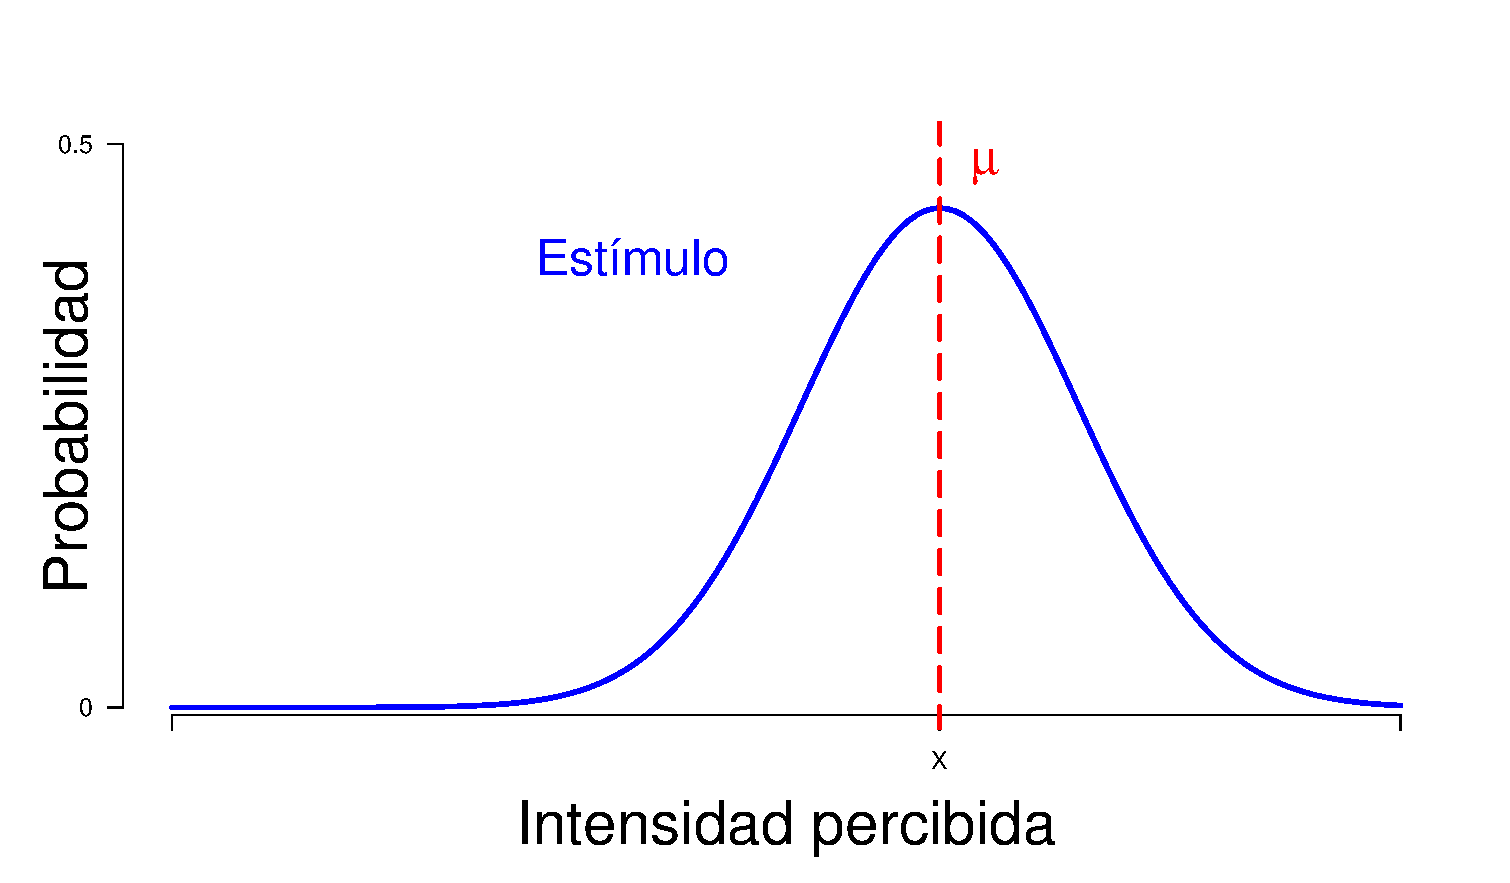
\includegraphics[width=0.75\textwidth]{Figures/Signal_Perception} 
\decoRule
\caption[Variabilidad en la percepción de los estímulos]{La variabilidad en la percepción de los estímulos es ilustrada con una distribución de probabilidad normal: al presentar un estímulo con intensidad $x$ en repetidas ocasiones, es muy probable que el valor percibido se acerque a su valor real (la media, $\mu$), pero también puede percibirse con mayor o menor intensidad.}
\label{fig:Senal_percepcion}
\end{figure}

\item Un psicólogo aplica una prueba clínica \textit{A} para evaluar si su paciente tiene depresión. Por lo general, las pruebas clínicas arrojan un puntaje \textit{p} que, de acuerdo a su correspondencia con el rango de puntajes típicamente obtenidos por personas que tienen cierta condición, sugieren el diagnóstico a emitir. La Figura~\ref{fig:Senal_presentacion}, presenta la idea central de este ejemplo: no todas las personas con depresión obtienen exactamente el mismo puntaje, sino que dentro de la serie de posibles puntajes a obtener en la prueba (todos los valores en el eje de las x), las personas con depresión suelen obtener resultados dentro de un rango específico con cierta probabilidad (la distribución azul), de tal suerte que hay puntajes que se asocian con dicha condición con mayor probabilidad (siendo la media de la distribución, $\mu$, señalada en rojo la más probable), que otros. También existe variabilidad en la presentación de ciertos estímulos en el entorno.\\
\end{itemize}

\begin{figure}[h]
\centering
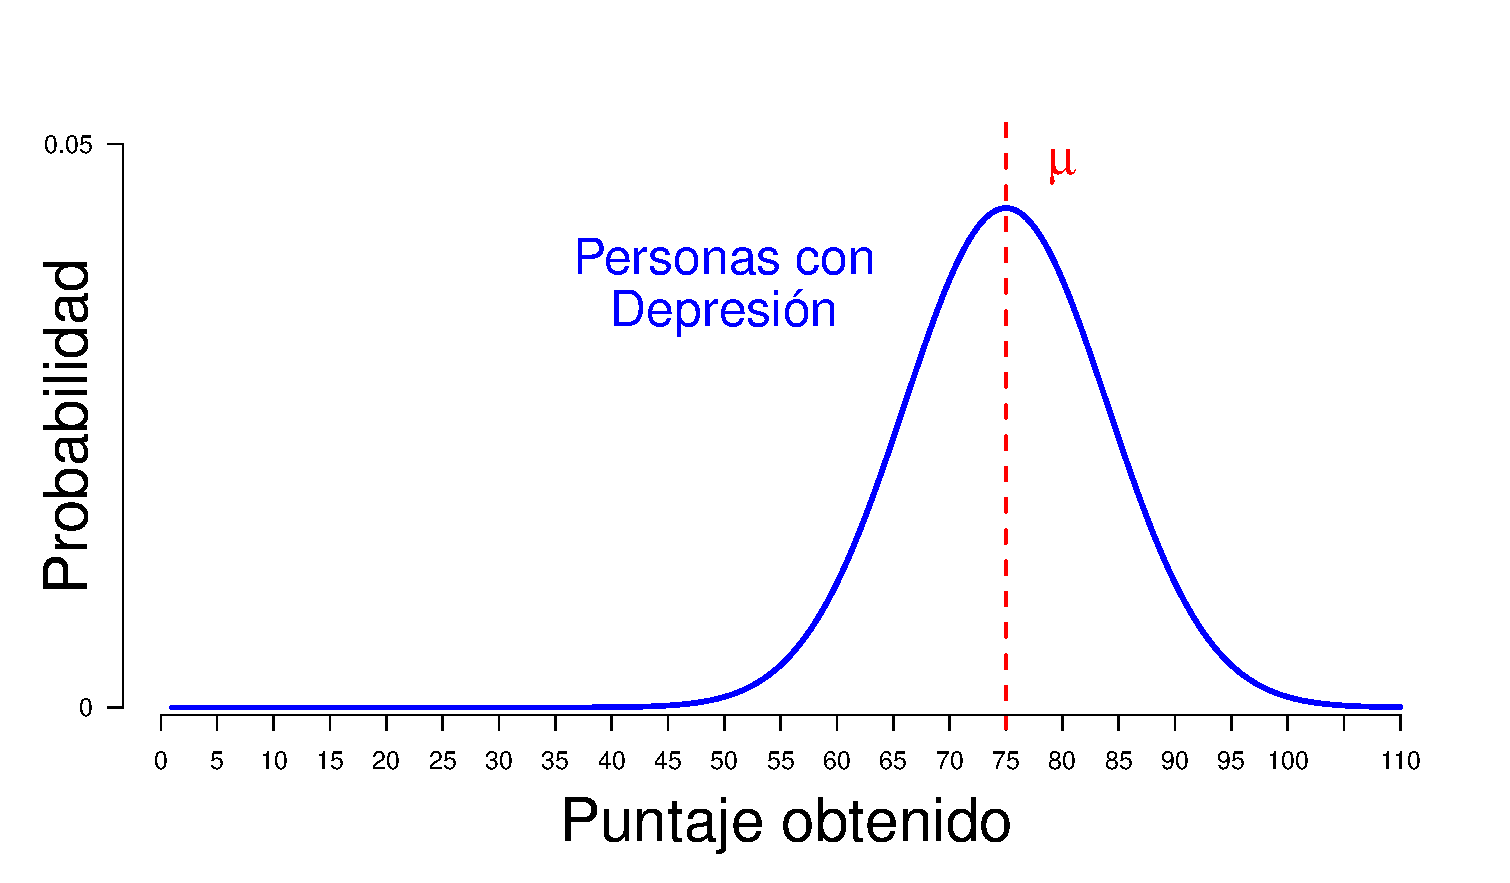
\includegraphics[width=0.75\textwidth]{Figures/Signal_Presentation} 
\decoRule
\caption[Variabilidad en la presentación de los estímulos]{La variabilidad en la presentación de los estímulos es representada con una distribución de probabilidad normal: En una prueba clínica de Depresión, las personas con dicha condición (la Señal) obtienen puntajes dentro de un rango de valores, con mayor o menor probabilidad al rededor de una media ($\mu$, señalada en rojo). Los valores presentados son arbitrarios.}
\label{fig:Senal_presentacion}
\end{figure}

En general, las Figuras~\ref{fig:Senal_percepcion} y \ref{fig:Senal_presentacion} ilustran un elemento fundamental en la forma en que la SDT concibe la detección de señales como un problema de adaptabilidad: la variabilidad es intrínseca a la percepción de los estímulos, ya sea porque nuestros sistemas sensoriales no los capturan igual en cada presentación, o porque los estímulos no se nos presentan exactamente de la misma forma en cada ocasión. Es otras palabras, los estímulos en cuya detección están interesados los organismos (las señales) son intrínsecamente variables (Tanner y Swets, \citeyear{Tanner1954}).\\

    \underline{b) La variabilidad en el Entorno: Ruido}\\

%La señal coexiste con el ruido y puede llegar a confundirse con el mismo.
Además del hecho de que existe variabilidad implícita en las señales a detectar, es necesario tomar en cuenta que estas coexisten en el mundo con otros estímulos o estados que -dada su propia variabilidad- pueden llegar a producir evidencia similar y confundir el diagnóstico de detección emitido por los organismos implicados en la tarea (Tanner y Swets, \citeyear{Tanner1954}). Esta misma idea fue propuesta por primera vez por Thurstone (\citeyear{Thurstone1927}), quien desarrolló un modelo estadístico para dar cuenta del problema que supone la discriminación entre dos estímulos, tomando en cuenta la variabilidad en la percepción y presentación de estos, una idea que posteriormente sería ampliamente desarrollada en Psicofísica (Swets, \citeyear{Swets1973}).\\

\begin{figure}[h]
\centering
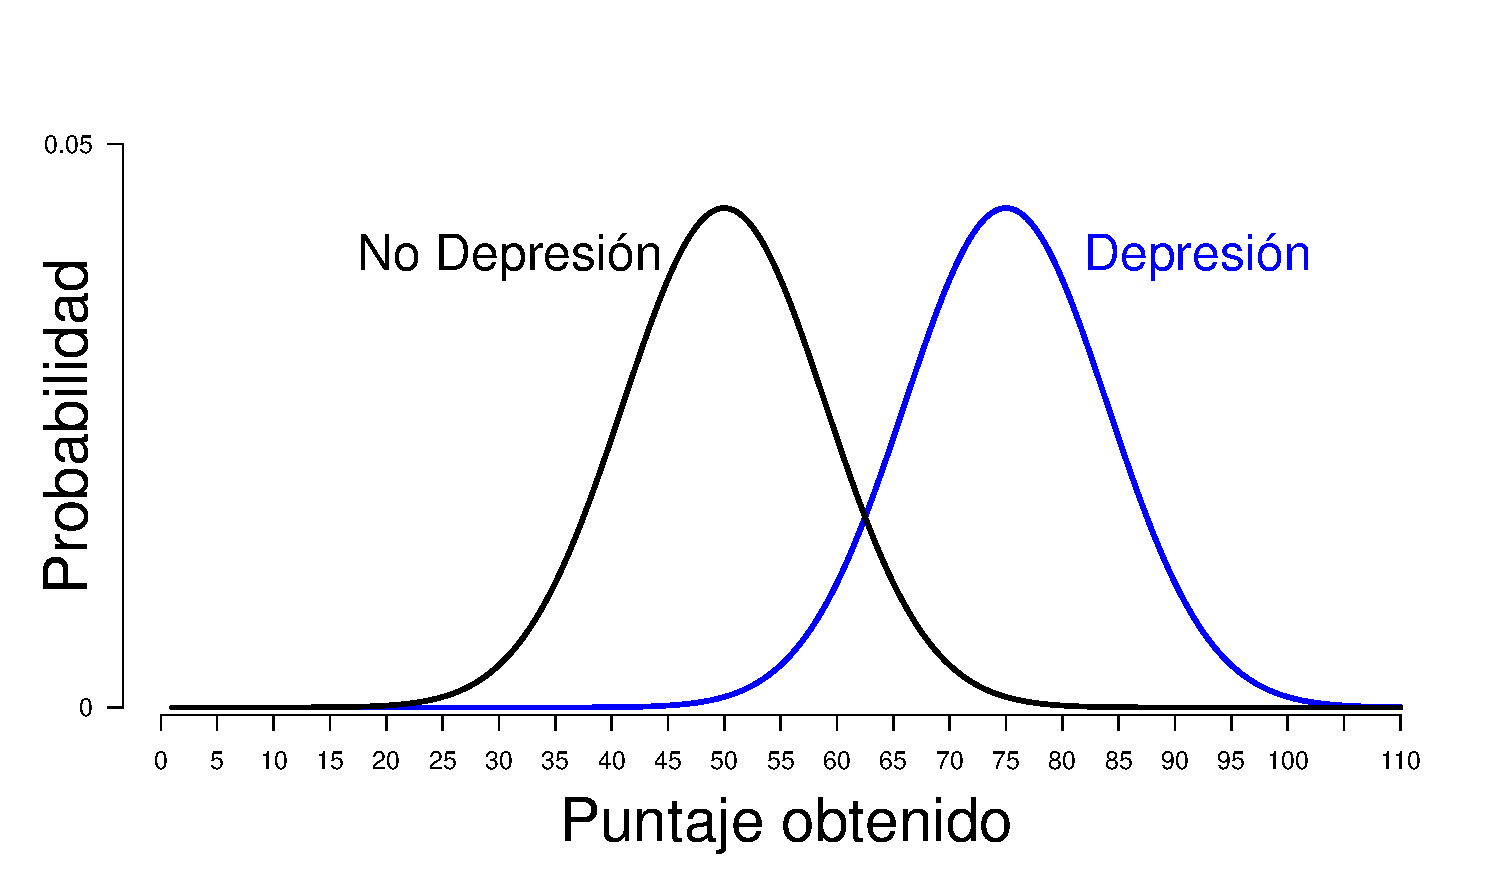
\includegraphics[width=0.75\textwidth]{Figures/Noise} 
\decoRule
\caption[Variabilidad en la señal y en el ruido]{Extensión del ejemplo sobre la variabilidad en los puntajes obtenidos en una prueba clínica por pacientes con depresión, donde además de la distribución asociada a la señal (en azul), se añade una distribución que representa los puntajes registrados por personas que no tienen depresión (el ruido; en negro). El sobrelape entre ambas distribuciones ilustra la incertidumbre contenida en la tarea.}
\label{fig:Noise}
\end{figure}

Retomando el ejemplo ilustrado en la Figura~\ref{fig:Senal_presentacion} sobre la variabilidad en los puntajes obtenidos en una prueba clínica por personas con depresión, en la Figura~\ref{fig:Noise} se agrega un segundo punto clave en la concepción de la detección de señales como un problema de decisión: también existe variabilidad en los puntajes obtenidos por las personas que responden la prueba sin tener dicha condición, con su propia distribución de probabilidad (en color negro). Nótese que ahora existe un sub-rango de valores donde las dos distribuciones se sobrelapan y recordemos que el objetivo de aplicar estas pruebas es detectar -\textit{diagnosticar}- la depresión -la señal- con base en el resultado obtenido por el paciente evaluado, ¿Cuál sería el diagnóstico pertinente para una persona que obtuvo un puntaje dentro del área de sobrelape? De acuerdo con la SDT, la forma ideal de resolver este conflicto -asumiendo que se conocen las distribuciones que subyacen al desempeño de las personas con y sin depresión- es optar por el juicio de elección \texit{más probable} a la luz de los datos (es decir, el que tenga una mayor densidad de probabilidad a la altura del puntaje registrado). El problema es claro: en tanto que la señal y el ruido pueden llegar a producir la misma evidencia, los sistemas detectores no pueden tener certeza absoluta sobre el juicio de detección a emitir y en su lugar, deben elegir aquel que les permita optimizar su comportamiento.\\ 

En el marco de la SDT, la discriminabilidad en las tareas de detección se define mediante la proporción de evidencia que comparten la señal y el ruido (es decir, \textit{'¿qué tan probable es que la señal y el ruido se confundan?'}), y en términos de la representación gráfica propuesta por la SDT, implica una evaluación de qué tan grande es el área de sobrelape entre las distribuciones, volviéndose esta el reflejo directo de la incertidumbre contenida en la tarea (\textit{'¿Qué tan discriminable -diferente- es la señal respecto del ruido?'}).\\

La Figura~\ref{fig:Overlap} presenta dos figuras representativas que ilustran la relación entre la distancia entre las distribuciones de Ruido y Señal -y el área de sobrelape entre estas- y su interpretación en términos de la discriminabilidad de los estímulos contenidos en la tarea. En el panel superior (a), las distribuciones están muy separadas y el sobrelape entre estas es pequeño, sugiriendo un entorno con poca incertidumbre donde es muy poco probable encontrar evidencia que pueda confundir al organismo -\textit{discriminabilidad alta}-. Por otro lado, si las distribuciones están más juntas, como ocurre en el panel inferior (b), el sobrelape será más grande y habrá un mayor rango de evidencia que se vincule simultáneamente con ambos estados del mundo, dificultando la emisión del juicio de detección adecuado -\textit{discriminabilidad baja}-.\\

\begin{figure}[h]
\centering
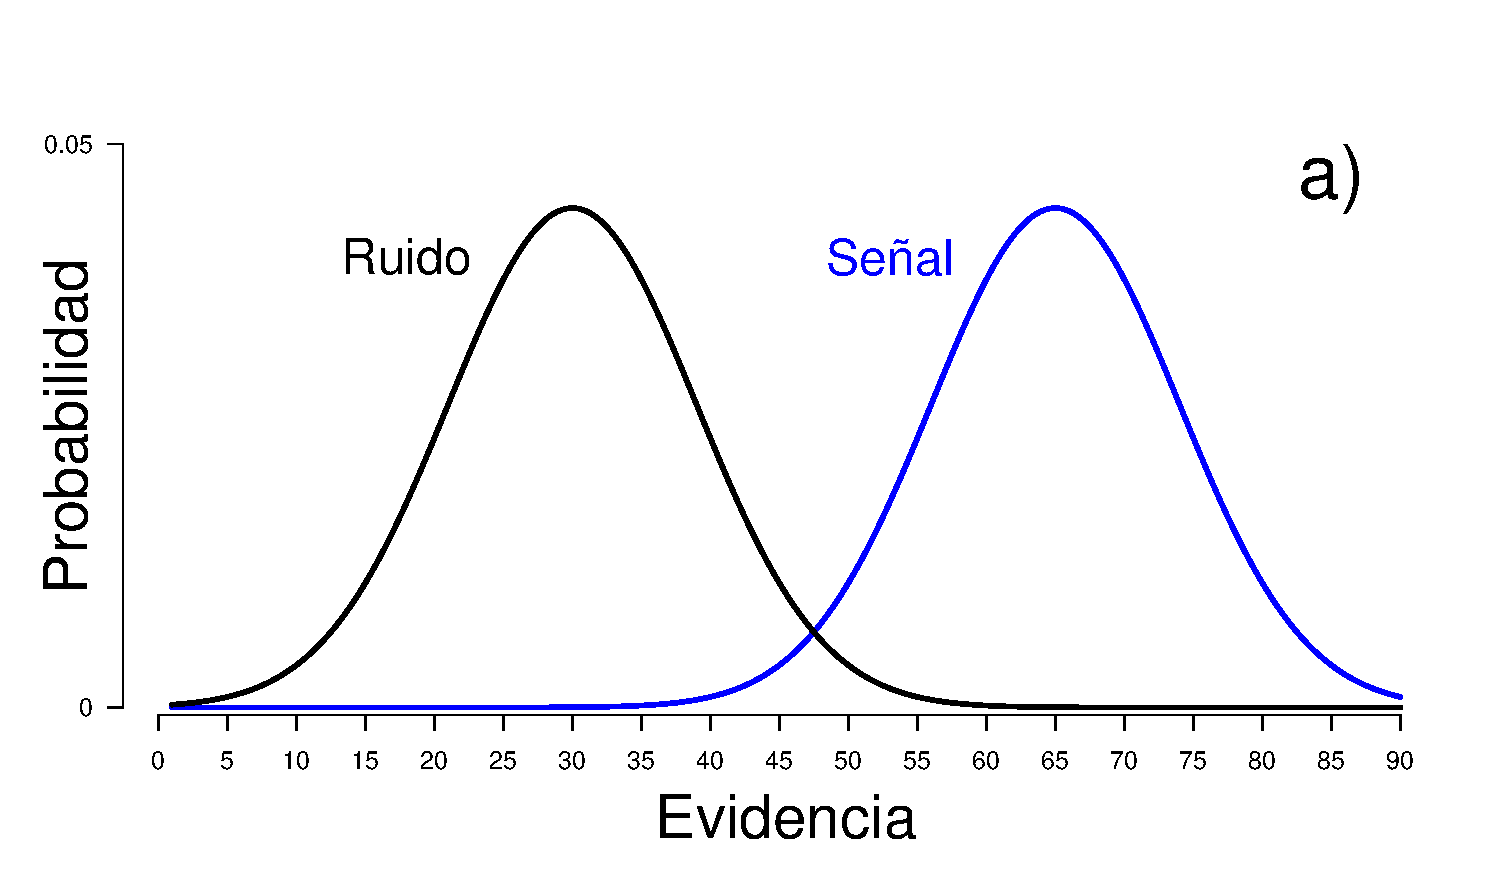
\includegraphics[width=0.65\textwidth]{Figures/Overlap_Small}\\ 
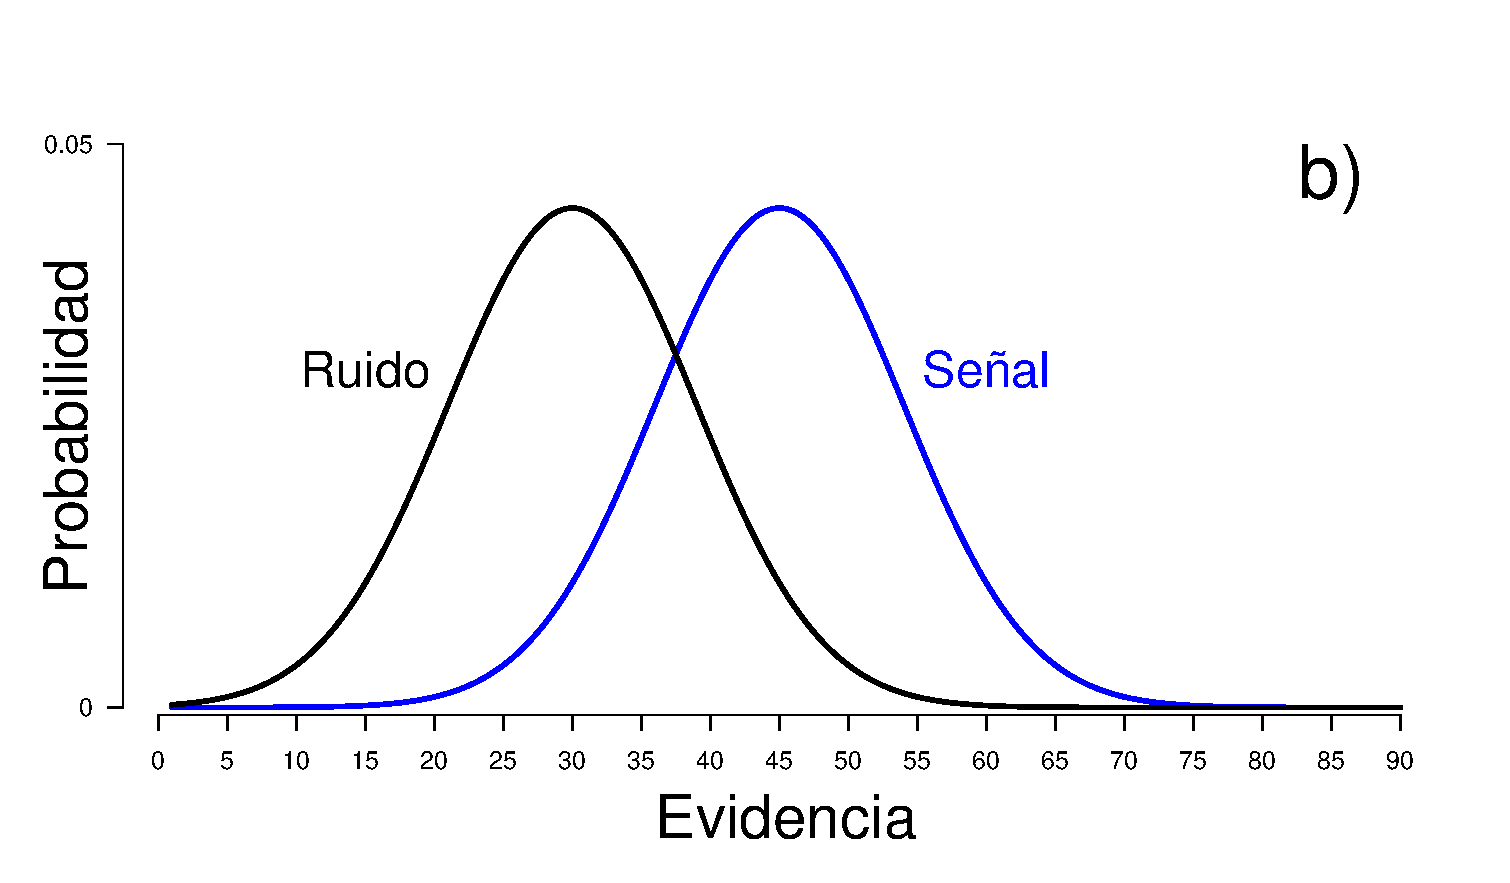
\includegraphics[width=0.65\textwidth]{Figures/Overlap_Big} 
\decoRule
\caption[La detección como una tarea con incertidumbre: el sobrelape entre las distribuciones]{La distancia entre las distribuciones de ruido y señal determina el sobrelape entre las mismas y por tanto, la incertidumbre contenida en la tarea. En el panel a) las distribuciones aparecen muy separadas y se asume poca incertidumbre.  En el panel b) se presenta un escenaro con mayor incertidumbre, siendo que el sobrelape entre las distribuciones es mayor.}
\label{fig:Overlap}
\end{figure}

La Discriminabilidad en una tarea de detección es producto de la variabilidad con que los posibles estados del mundo se presentan y perciben por los sistemas detectores. Es decir, depende tanto de las propiedades intrínsecas de los estímulos a evaluar -\textit{¿Qué tanto parecido tienen los estímulos con la señal y los estímulos sin esta?}- como de la precisión con que los sistemas detectores son capaces de discernir entre dichas instancias -\textit{¿Qué tan bueno es el organismo para distinguir una señal del ruido?}- (Nevin, \citeyear{Nevin1969}). Por ejemplo, no es lo mismo tratar de detectar una manzana entre un montón de naranjas que entre un montón de melocotones, (en general, esperaríamos que la tarea fuera más sencilla en el primer escenario al tener una mayor discriminabilidad); de la misma forma, la tarea de detectar si un instrumento musical está desafinado no es igual de difícil para un músico que para una persona sin educación musical.\\

  \textbf{2.- El papel del Sesgo: La detección es decisión}\\

La variabilidad en la presentación y percepción de los eventos en el mundo constituye el elemento clave para entender la detección de señales como una problema cargado de incertidumbre, donde no se puede confiar completamente en la evidencia presente para emitir un juicio de detección. De acuerdo con la SDT, los organismos compensan la incertidumbre contenida en las tareas de detección con la información que poseen sobre el entorno que, en términos generales, puede ser de dos tipos: 1) información probabilística e 2) información sobre las consecuencias comprometidas (Nevin, \citeyear{Nevin1969}).\\

Como ejemplo, tomemos el caso de un médico que trata de decidir si los resultados obtenidos en cierta prueba clínica son evidencia suficiente para diagnosticar una enfermedad \textit{X} a un paciente \textit{Y}. La evidencia con la que el médico cuenta es imprecisa: toda prueba clínica tiene un margen de error y su lectura debe complementarse con la historia clínica del paciente; el médico debe tomar en cuenta toda la información de la que dispone: \textit{¿Qué tan confiable es la prueba?}, \textit{¿Cuál es su tasa de aciertos y errores?}; \textit{¿Qué tan común es la enfermedad que intenta detectar?} y \textit{¿Qué tan probable es que el paciente Y tenga dicha enfermedad de acuerdo con los factores de riesgo asociados a la misma?}. Y aún ponderando toda esta información, el problema no termina aquí. La información probabilística permite hacer inferencias sobre cuál es la conclusión más \textit{probable}, pero sigue sin haber certeza sobre el diagnóstico. Para optimizar su comportamiento y tomar la mejor decisión posible, el médico también debe tomar en consideración la información que posee sobre las consecuencias asociadas a cada escenario posible: a) Si el paciente tiene la enfermedad y el médico la detecta acertadamente, podrá tratarse a tiempo; b) Si tiene la enfermedad y el médico falla en detectarla, podría poner en riesgo su vida; c) Si no tiene la enfermedad y el médico le dice que sí, se gastarán recursos innecesarios en solucionar un problema que no existe, corriendo el riesgo de que el tratamiento le haga daño y d) Si no tiene la enfermedad y el médico decide no darle el diagnóstico, todo permanecerá igual. La tarea del médico es mucho más compleja de lo que parecía en un principio, puesto que no se limita a la lectura de la prueba clínica, sino que tiene que ponderar lo que sugieren los resultados de la misma con toda la información que posee sobre la probabilidad de las interpretaciones posibles y las consecuencias comprometidas.\\

\begin{figure}[h]
\centering
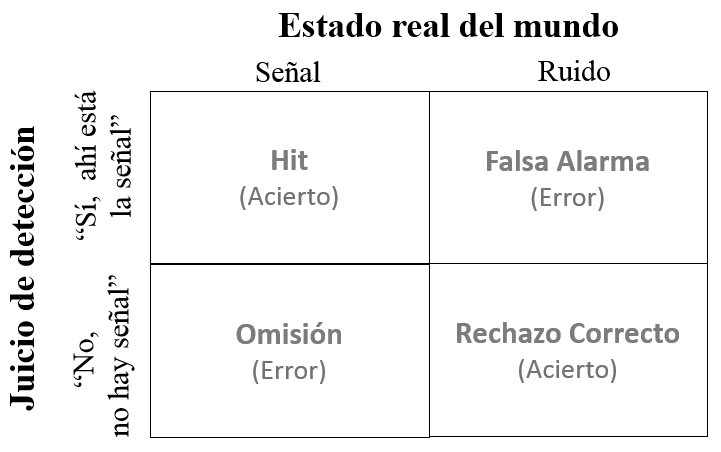
\includegraphics[width=0.65\textwidth]{Figures/Matriz_Outputs} 
\decoRule
\caption[Matriz de contingencia: Resultados a obtener en una tarea de detección]{Los cuatro posibles resultados a obtener en una tarea de detección de señales, de acuerdo con la correspondencia entre el juicio emitido y el estado del mundo.}
\label{fig:Mat_Output}
\end{figure}

De acuerdo con la correspondencia entre el \textit{estado real del mundo} -la presencia o ausencia de la señal- y el juicio emitido por el sistema detector, la SDT distingue entre dos tipos de aciertos y errores, ilustrados en la Figura~\ref{fig:Mat_Output} con una Matriz de contingencia. Cuando la señal está presente el organismo puede detectarla adecuadamente (un \textbf{Hit}) o dejarla pasar (una \textbf{Omisión}); y si por el contrario, la señal no está presente, el organismo puede acertar al diagnosticar su ausencia (un \textbf{Rechazo Correcto}) o confundir el ruido con la señal, (una \textbf{Falsa Alarma}).\\

La SDT asume que el organismo fija un criterio de elección para determinar a partir de cuánta evidencia va a juzgar la presencia de la señal, con base en la informació que posee sobre la probabilidad de que ésta ocurra y las consecuencias comprometidas en su detección (Tanner y Swets, \citeyear{Tanner1954}; Swets y cols., \citeyear{Swets1961}; Nevin, \citeyear{Nevin1969}). En términos de la representación gráfica del modelo, el criterio se concibe como una línea vertical que atraviesa las distribuciones de ruido y señal (como se ilustra en color rojo en la Figura~\ref{fig:Graf_Outputs}), para definir a partir de cuánta evidencia se emitirá un juicio de detección afirmativo.

\begin{figure}[bh]
\centering
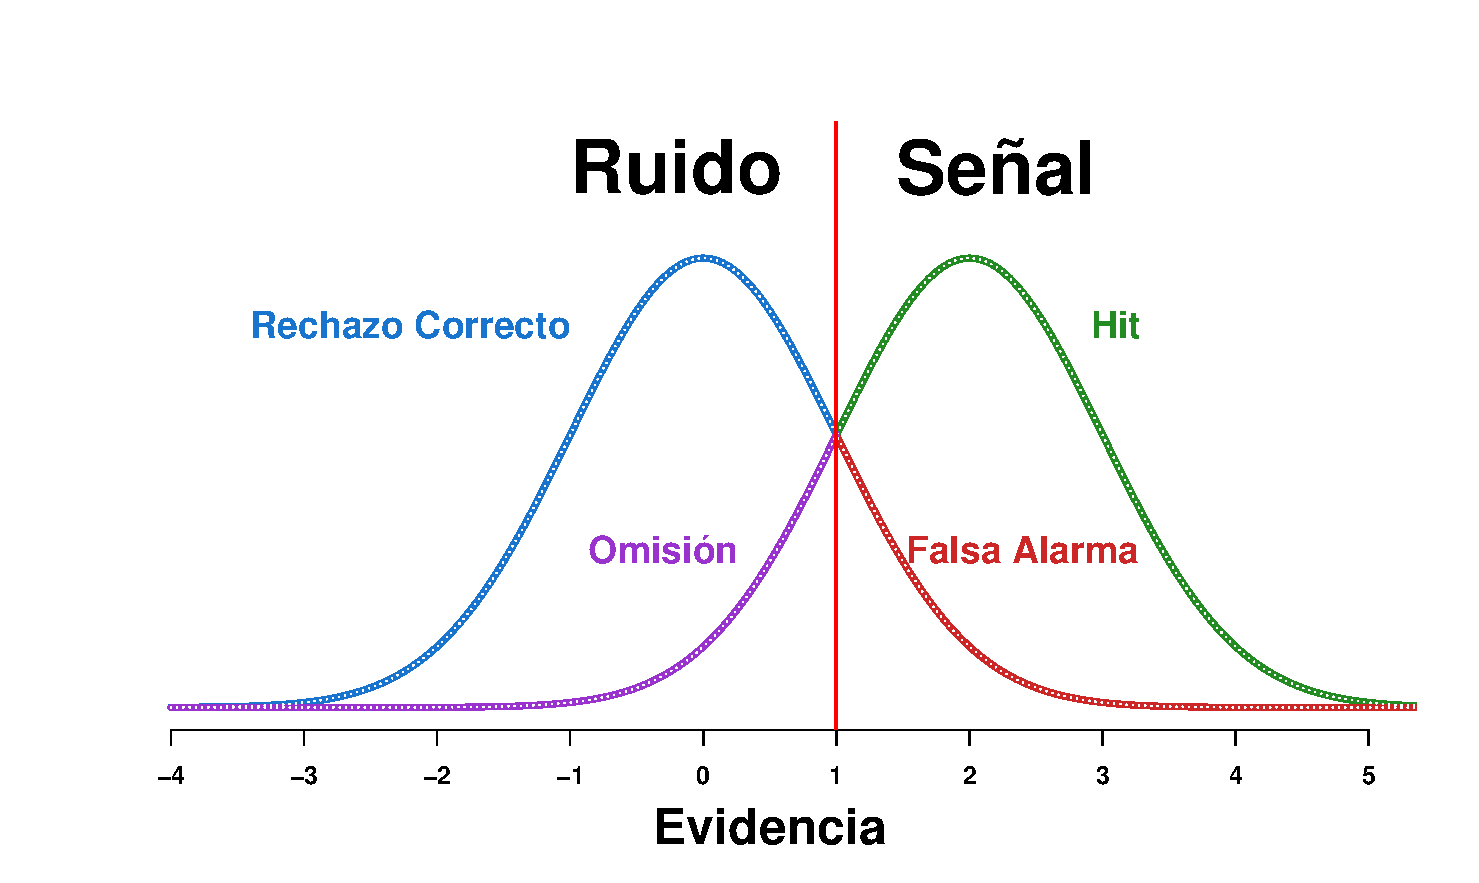
\includegraphics[width=0.8\textwidth]{Figures/SDT_OutcomesR} 
\decoRule
\caption[Representación gráfica de las tareas de detección y los posibles resultados a obtener]{Representación gráfica de los problemas de detección de acuerdo con la SDT: existen distribuciones de probabilidad que describen la variabilidad con que las señales y el ruido se presentan, con un área de traslape que refleja la incertidumbre en la tarea. El criterio de elección fijado por el organismo (línea roja) determina a partir de cuánta evidencia se juzgará la presencia de la señal y cuál es la probabilidad de cometer un acierto o error (en colores).}
\label{fig:Graf_Outputs}
\end{figure}

La Figura~\ref{fig:Graf_Outputs} presenta la representación final de los problemas de detección bajo el marco de la SDT: se tienen dos distribuciones de probabilidad que representan la variabilidad con que la señal y el ruido ocurren en el ambiente y una línea roja que señala el criterio que el sistema detector va a utilizar para emitir sus juicios de detección. Como se ilustra con distintos colores en la figura, la localización del criterio determina la probabilidad con que el organismo podría incurrir en cada uno de los resultados expuestos previamente en la figura~\ref{fig:Mat_Output}.\\

De acuerdo a la estructura de la tarea y al conocimiento que los organismo tengan sobre ella, es posible que se desarrolle un \textit{sesgo} de elección que lleve a favorecer -\textit{hacer más propensa}- la emisión de un juicio de detección particular (Nevin, \citeyear{Nevin1969}). De esta forma, la localización del criterio sobre el eje de evidencia es un reflejo directo de este sesgo, que puede variar en función de dos grandes factores:\\

      \underline{a) Los errores cuestan y los aciertos pagan: Matrices de pago}\\

La variabilidad asociada a los estímulos en el ambiente da pie a que los sistemas involucrados en tareas de detección de señales cometan errores. Tomando en cuenta que las señales son estímulos relevantes para el sistema, en tanto que permiten dirigir su comportamiento en función de las relaciones de contingencia anunciadas con su detección, acertar o errar en el juicio emitido tiene consecuencias importantes. Los aciertos pagan y los errores cuestan, y más aún, cada uno lo hace con distinta magnitud.\\

Imaginemos el caso de un conejo que tiene que decidir, tan rápido como pueda, si el sonido que acaba de escuchar en la maleza corresponde o no, con el de un depredador. La penalización por cometer una Falsa Alarma -un gasto innecesario de energía al correr por nada- es sustancialmente diferente al precio que tendría que pagar por una Omisión -¡la muerte!-. Dadas las consecuencias en juego, es muy probable que el conejo emita un juicio de detección afirmativo (\textit{'¡Sí, es un depredador!'}) y corra por su vida, aún con muy poca evidencia.\\

\begin{figure}[h]
\centering
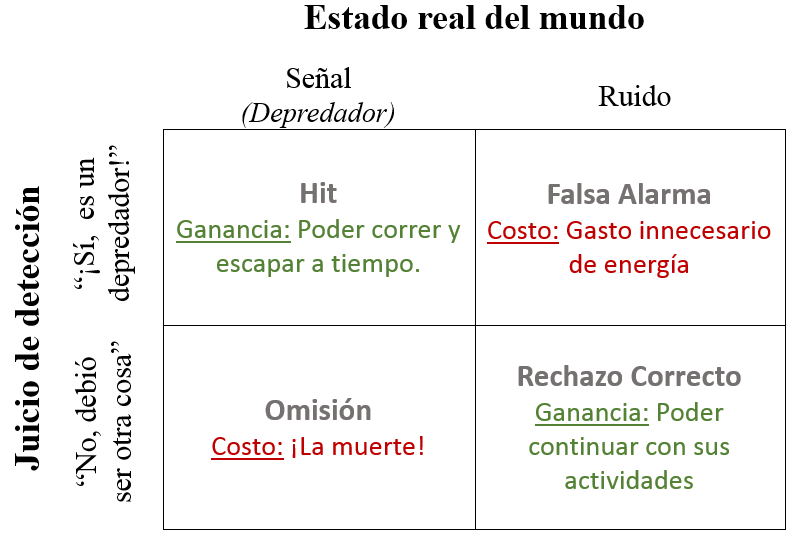
\includegraphics[width=0.7\textwidth]{Figures/Matriz_Pagos} 
\decoRule
\caption[Matriz de Pagos: Consecuencias comprometidas en una tarea de detección hipotética (ejemplo)]{Matriz de pagos con los costos y ganancias comprometidos en la tarea de detectar un depredador.}
\label{fig:Mat_Pagos}
\end{figure}

La figura~\ref{fig:Mat_Pagos} presenta lo que en los modelos clásicos de decisión se conoce como \textit{Matriz de Pagos} y que se utiliza para señalar, de acuerdo a una matriz de contingencia, los costos y ganancias asociados con las tareas de detección. De acuerdo con la SDT, ya que no se puede tener certeza absoluta sobre el juicios de detección a emitir, la evidencia es juzgada en función a un criterio de elección que toma en cuenta las consecuencias comprometidas en su entorno, para guiar de manera óptima el comportamiento del organismo (Killeen, \citeyear{Killeen2014}).\\

      \underline{b) Estimados de Probabilidad}\\

Los organismos inmersos en tareas de detección tienen expectativas sobre la probabilidad de observar una señal en su entorno. Ya sea como resultado de su experiencia directa con el mundo, o porque es información que les ha sido proporcionada de manera externa (Nevin, \citeyear{Nevin1969}), los agentes detectores tienen alguna idea o conocimiento sobre la estructura probabilística de la tarea a resolver, en dos sentidos: 

\begin{itemize}
\item \textsl{Un estimado prior.} Con independencia de cuál sea la evidencia evaluada de manera inmediata, \textit{¿Qué tan probable es encontrar la señal en esta situación particular?}\\

Si los organismos se encuentran en un entorno donde saben que es prácticamente imposible encontrar la señal, es muy probable que decidan descartar la evidencia que se les presente aún cuando correlacione con lo que se esperaría de una señal. Recordemos el ejemplo planteado anteriormente sobre el querer determinar la edad de una persona con la que hablamos por teléfono: si la llamada fue hecha a un despacho de abogados -o cualquier otro escenario donde se piense que es muy poco probable encontrar a un niño-, y la persona al otro lado del teléfono tiene una voz muy aguda, es muy poco probable que se decida pensar \textit{'Oh, estoy hablando con un niño'}.\\

\item \textsl{La verosimilitud.} Dado lo que se sabe sobre cómo se presentan los estímulos en el entorno, \textit{¿qué tan verosímil es la evidencia?} o bien, \textit{¿qué tan probable es que la señal se presente con la evidencia presente?}\\

Una vez que los organismos han adquirido información suficiente sobre su entorno -o una tarea particular- y conocen la variabilidad con que la señal y el ruido aparecen, los juicios de detección pueden ser emitidos a partir del cómputo de una razón de verosimilitud que permita al organismo estimar cuál es el estado del mundo con que la evidencia incierta se relaciona con mayor probabilidad. Es decir que, en términos de la representación gráfica del modelo, se asume que cuando los organismos se enfrentan a evidencia que cae en el área de sobrelape entre las distribuciones, optarían por elegir el juicio de detección que corresponda con la distribución que tenga una mayor densidad de probabilidad (es decir, la distribución que sea más alta en ese punto particular del eje de decisión) (Nevin, \citeyear{Nevin1969}).\\
\end{itemize}

De contar con un estimado prior y un buen conocimiento sobre las funciones de verosimilitud, es posible suponer que los organismos opten por el juicio de detección que resulte más probable, con base en el cómputo de una inferencia bayesiana (Ma, \citeyear{WeijiMa}; Ma, Kording y Goldreich \citeyear{WeijiMa2012}; Pouget, BEck, Ma y Latham, \citeyear{Pouget2013}).\\

\subsection{Parámetros del modelo}\\

La SDT, además de proporcionar un modelo estadístico para comprender las implicaciones adaptativas de los problemas de detección, funge como una herramienta que -dados los supuestos que hace sobre este tipo de tareas- permite hacer estimaciones sobre la discriminabilidad y el sesgo de sistemas inmersos en tareas de detección experimentales (Stainslaw y Todorov, \citeyear{Stainslaw1999}; McNicol, \citeyear{McNicol1}).\\

Las tareas de detección diseñadas en el laboratorio suelen estar compuestas por un amplio número de ensayos, a lo largo de los cuales se presenta aleatoriamente la señal o el ruido y se les solicita a los participantes que emitan un juicio de detección. Dependiendo el objetivo del estudio realizado, se pueden implementar manipulaciones adicionales (Nevin, \citeyear{Nevin1969}), o utilizar distintos protocolos en la presentación de la tarea de detección, (descritos en detalle en la \textbf{Sección 2.1.3}; McNicol, \citeyear{McNicol2}).\\

Al someter un sistema a una misma tarea de detección en repetidas ocasiones (como ocurre en las tareas experimentales), se espera encontrar variabilidad en los resultados obtenidos: el sistema no acertará o errará siempre, la evidencia evaluada no rebasará el criterio de elección en todos los ensayos a causa de la variabilidad en los estímulos (Wickens, \citeyear{Wickens1}. A partir del número de aciertos y errores cometidos en los ensayos con Ruido y Señal, se computan las tasas con que se obtuvieron cada uno de los resultados posibles. Dentro del total de veces que se presentó la señal, se identifica cuántas veces se cometió un Hit o una Omisión, y dentro del total de veces que se presetó sólo el Ruido, la proporción de ensayos en que el participante hizo un Rechazo Correcto o una Falsa Alarma.\\

De acuerdo con la SDT clásica, las tasas registradas en tareas de detección son reflejo del área de las distribuciones de Ruido y Señal que caen a cada lado del criterio y por lo tanto, pueden utilizarse para hacer inferencias sobre la localización del mismo, la distancia entre las distribuciones y la preferencia que podría tener el sistema por emitir una respuesta sobre otra (Wickens, \citeyear{Wickens1}; McNicol, \citeyear{McNicol1}; Gesheider, \citeyear{Gescheider}). A continuación, revisaremos en detalle cuáles son los parámetros incluidos en el modelo de detección de señales.\\

  \textbf{Supuestos formales}\\

La estimación paramétrica del modelo de detección de señales se desarrolla en torno a una serie de supuestos formales -especificaciones técnicas- que facilitan la interpretación de los datos obtenidos a la luz de la representación gráfica propuesta por la SDT (Wickens, \citeyear{Wickens1}; Gescheider, \citeyear{Gescheider}; Stainslaw y Todorov, \citeyear{Stainslaw1999}).\\ 

\begin{enumerate}

\item  Dado que las cuatro tasas de ejecución se computan en función a dos conjuntos -total de estímulos con Señal y Ruido-, sólo se necesita de un par de ellas para tener información completa sobre el desempeño de los participantes. Por ejemplo, por consenso general suelen reportarse sólo las tasas de Hits y Falsas Alarmas -los aciertos y errores obtenidos cuando el participante respondió \textit{'Sí, detecto la señal'}-, pues las tasas de Omisiones y Rechazos Correctos no son más que su complemento (Wickens, \citeyear{Wickens1}.\\

\item En su forma clásica, la SDT asume que las distribuciones de Ruido y Señal son distribuciones normales equivariantes (Stainslaw y Todorov, \citeyear{Stainslaw1999}).\\
  \begin{itemize}
  \item Se utilizan distribuciones normales como el \textit{default} para describir la variabilidad contenida en cualquier conjunto de estímulos Señal y Ruido, pero existe literatura que explora la conveniencia de representar la incertidumbre con otro tipo de distribuciones (Wickens, \citeyear{Wickens1}; Ma, \citeyear{WeijiMa2009}).\\
  \item En la mayoría de sus aplicaciones, se asume que las distribuciones de ruido y señal comparten una varianza de 1 (Tanner y Swets, \citeyear{Tanner1954}). No obstante, al aplicar la SDT al estudio de la memoria de reconocimiento, se ha encontrado evidencia consistente de que la distribución de señal tiene una varianza mayor que la del ruido (Wixted, \citeyear{Wixted2007}).\\
  \end{itemize}

\item Se asigna de manera arbitraria una media en 0 a la distribución de Ruido para facilitar el cómputo del resto de los parámetros, utilizando ésta como punto de referencia (Wickens, \citeyear{Wickens1}; \citeyear{Gescheider}).\\

\item Una de las implicaciones directas de la forma en que está constituida la SDT es que, sea cual sea la evidencia con base en la cual se estén formando los juicios de detección -los valores en el eje $X$ sobre el que se despliegan las distribuciones-, se espera que la señal tenga \textit{más} de ello que el ruido, en tanto que este último implica su ausencia (Stainslaw y Todorov, \citeyear{Stainslaw1999}).\\
  \begin{itemize}

  \item La tasa de Falsas Alarmas no puede ser más grande que la tasa de Hits. Esto implicaría que hay una mayor área de la distribución de ruido por encima del criterio que de la distribución de señal. Esto, a su vez, sugeriría que el ruido cae por encima de la señal y se estaría violando el supuesto fundamental de que la Señal -la presencia de lo que queremos detectar- contiene más información que el Ruido -su ausencia-.\\
  \end{itemize}
\end{enumerate}

Los parámetros contemplados por el modelo evalúan el desempeño de los participantes en términos de los dos grandes factores que se asocian con la emisión de juicios de detección: la discriminabilidad y el sesgo. La aplicación exitosa de la SDT al estudio de una amplia gama de tareas de detección -que pueden variar desde el tipo de estímulos utilizados hasta el dominio o fenómeno a estudiar- es posible gracias a la abstracción de sus elementos. Los valores y el tipo de evidencia específicos sobre los cuales se despliegan las distribuciones de Ruido y Señal no importan tanto -de hecho, no suelen tomarse en cuenta en lo absoluto- como saber qué tanto sobrelape hay entre las distribuciones y cuál es el juicio de detección que se prefiere emitir.\\

\pagebreak
\begin{itemize}
\item \underline{Criterio ($k$)}\\

La localización del criterio sobre el eje de decisión se puede computar de manera directa a partir de la tasa registrada de Rechazos Correctos, tomando como referencia la media asignada a la distribución de ruido ($0$). \\

El parámetro $k$ representa la localización del criterio sobre el eje de evidencia en unidades de \textit{desviación estándar} (Tanner y Swets, \citeyear{Tanner1954}). Su cómputo requiere interpretar la tasa de Falsas Alarmas como reflejo de la probabilidad acumulada -el área bajo la curva- por encima del criterio en la distribución de Ruido, siendo la tasa de Rechazos Correctos su complemento. Dado que la distribucion de ruido tiene media en 0 y desviación estándar de 1, la tasa de Rechazos Correctos (ó $1 - Tasa$ $F.A.$) puede ser transformada en \textit{Puntajes Z} para conocer la localización del criterio de elección sobre la distribución de ruido. Esto se realiza a partir del uso de la funcón matemática $\phi^{-1}$ (\textit{'phi inversa'}), que permite estimar conocer cuál es el Puntaje Z que corresponde con el punto donde se ha acumulado cierta densidad de probabilidad en una distribución normal estándar, (Stainslaw y Todorov, \citeyear{Stainslaw1999}).

\begin{figure}[h]
\centering
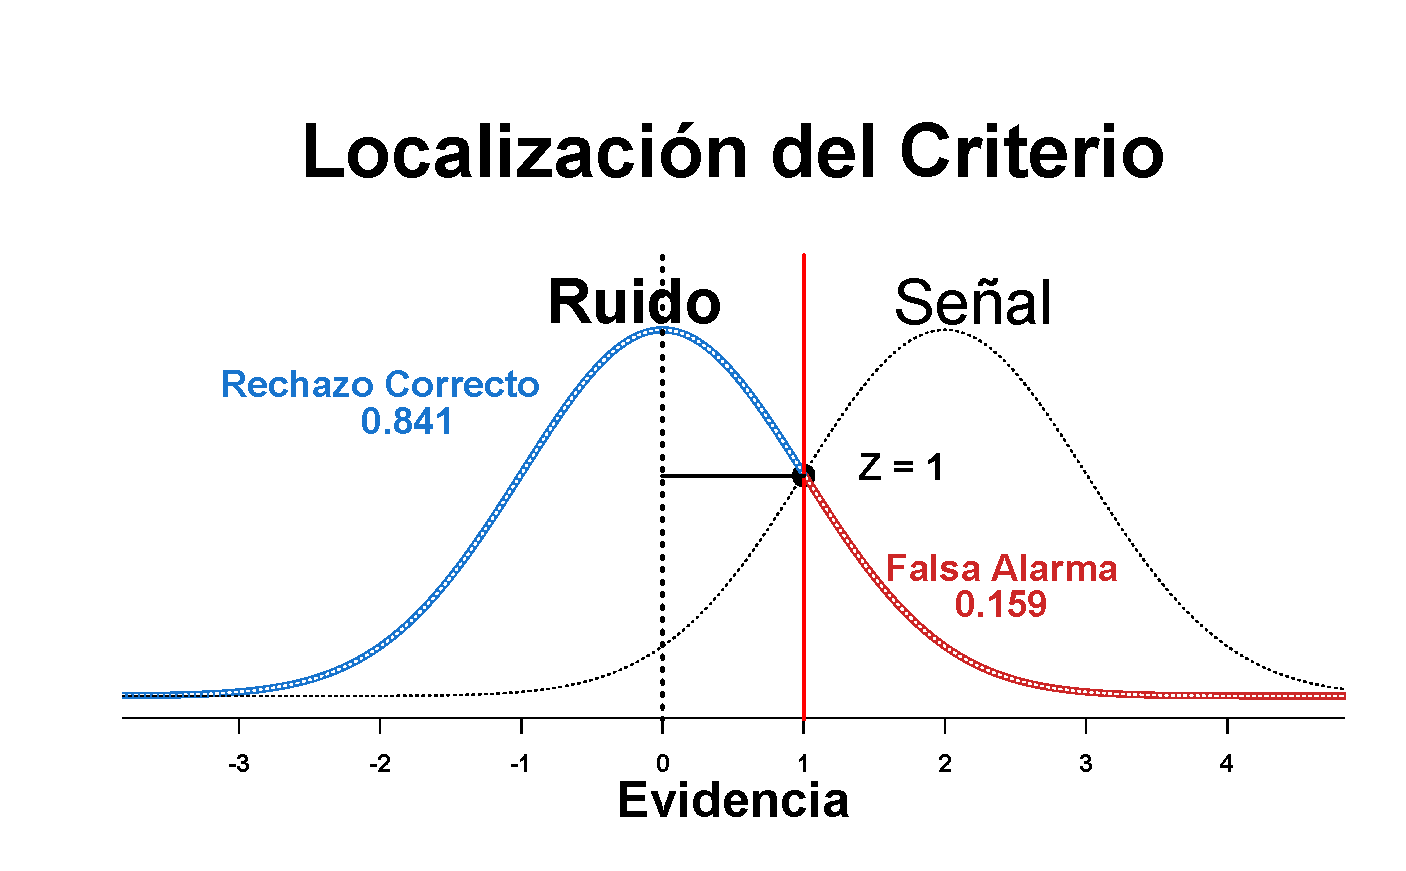
\includegraphics[width=0.75\textwidth]{Figures/Graficador_CriterioR} 
\decoRule
\caption[Estimación paramétrica: La localización del criterio]{Estimación de la localización del criterio sobre el eje de decisión con base en las tasas de Falsas Alarmas y Rechazos Correctos.}
\label{fig:Graf_Criterio}
\end{figure}

La Figura~\ref{fig:Graf_Criterio} ilustra la estimación de $k$ a partir de las tasas de Falsas Alarmas y Rechazos Correctos. Al transformar esta última en Puntajes Z, se puede establecer la ubicación del criterio respecto del 0 de referencia planteado por la media de la distribución de ruido (Stainslaw y Todorov, \citeyear{Stainslaw1999}). Es decir:

\begin{center}
$k = Z(Tasa$ $R.Correctos)$\\
donde $Z()$ representa una conversión a Puntajes Z.\\
\end{center}\\
\newline

\item \underline{Discriminabilidad ($d'$)}\\

La discriminabilidad de los estímulos comprometidos en una tarea de detección se cuantifica con un parámetro $d'$ que representa la distancia entre las medias de las distribuciones de ruido y señal, (Tanner y Swets, \citeyear{Tanner1954}). Dado que la distribución de ruido tiene media en 0, $d'$ también suele utilizarse para referir la ubicación de la media de la distribución de señal sobre el eje de evidencia, (McNicol, \citeyear{McNicol1}).\\ 

Una vez definida la localización del criterio relativa a la media de la distribución de ruido, es sencillo concebir el cómputo de $d'$ como una extensión de dicho procedimiento. Las tasas de Hits y Omisiones son utilizadas para establecer la localización de la media de la distribución de Señal sobre el eje de evidencia, a partir del criterio.\\ 

\begin{figure}[p]
\centering
%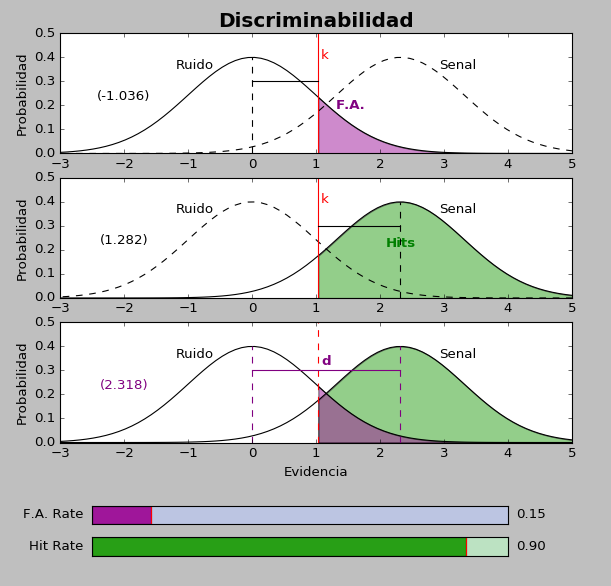
\includegraphics[width=0.80\textwidth]{Figures/Graficador_Discriminabilidad} 
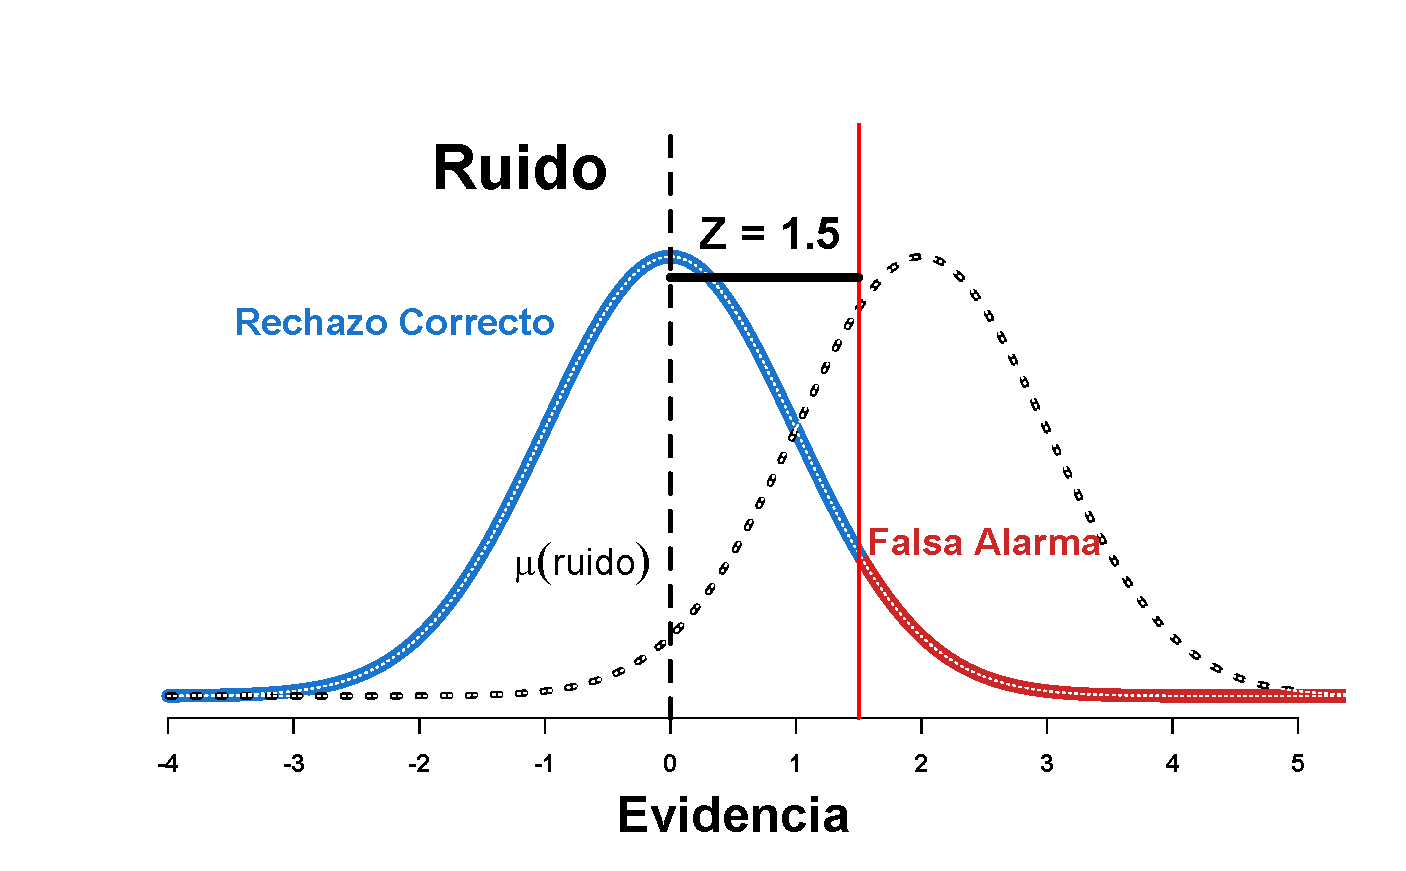
\includegraphics[width=0.65\textwidth]{Figures/dR_1} 
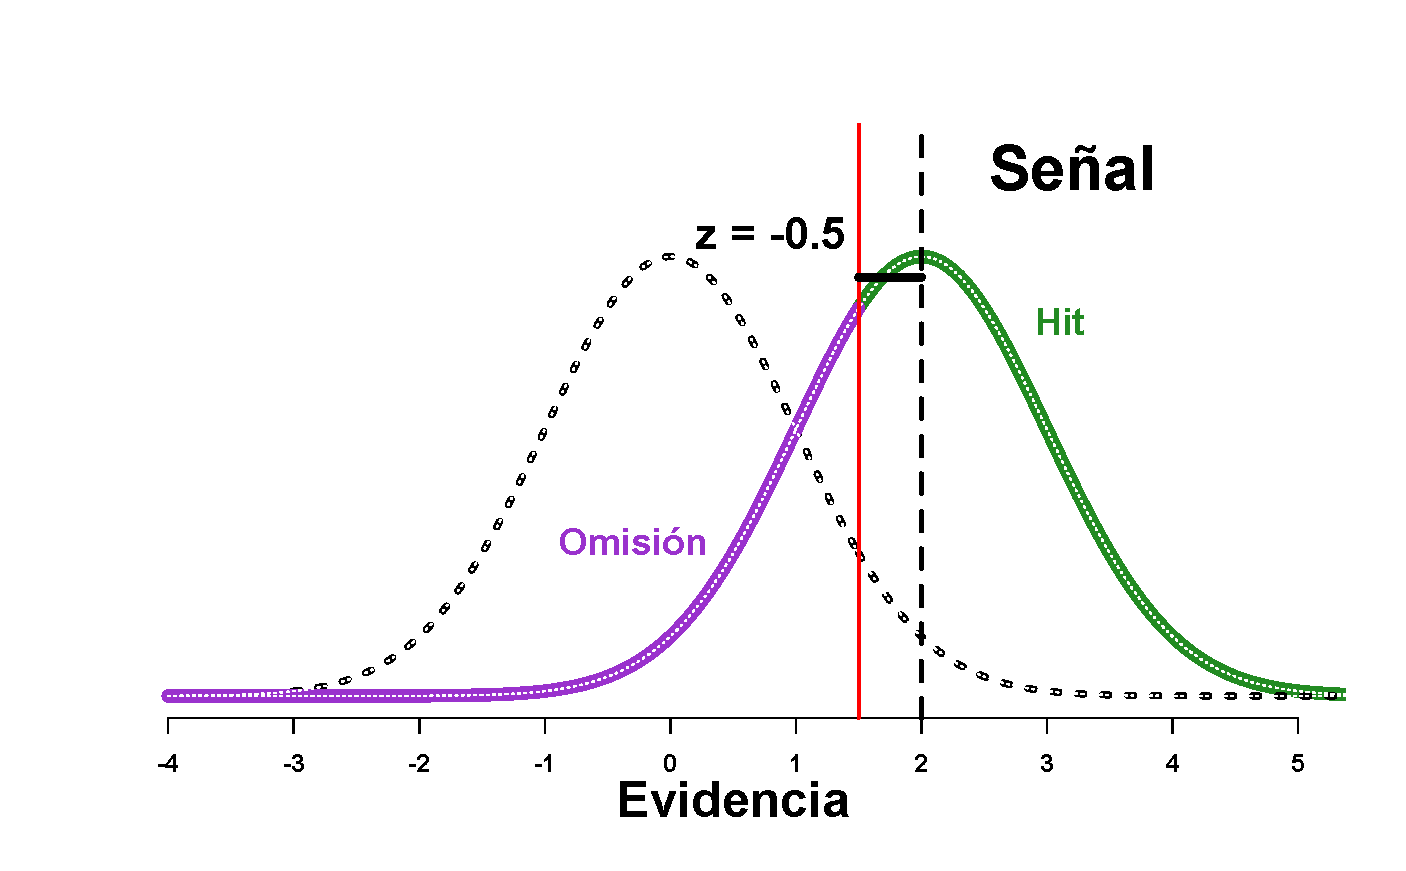
\includegraphics[width=0.65\textwidth]{Figures/dR_2}
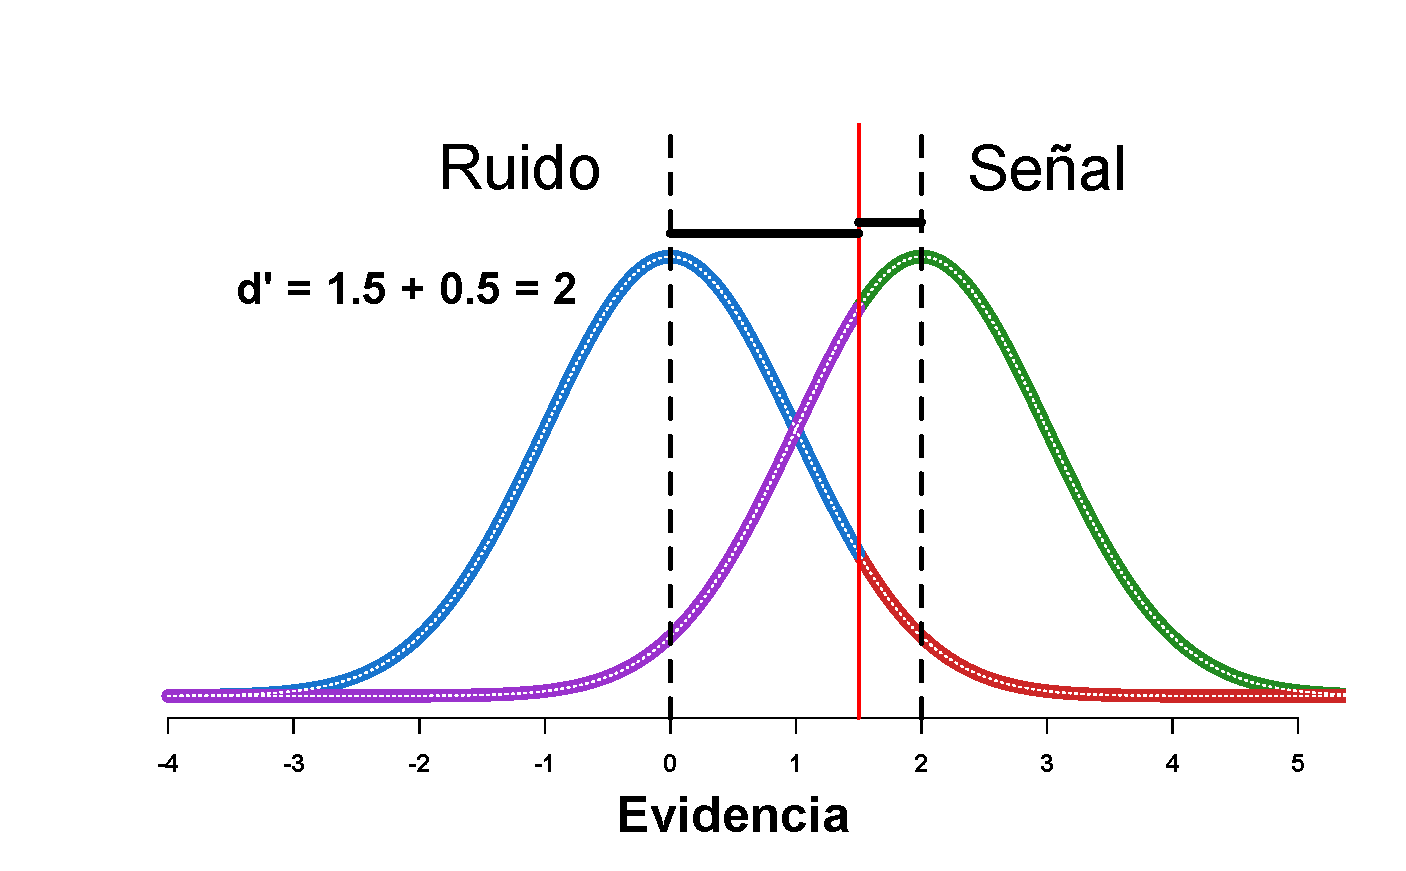
\includegraphics[width=0.65\textwidth]{Figures/dR_3}
\decoRule
\caption[Estimación paramétrica: la discriminabilidad ($d'$)]{Ilustración del cómputo de $d'$. Las tasas de Falsas Alarmas y Rechazos Correctos señalan la distancia entre el criterio y la media de la distribución de ruido (panel superior). Las tasas de Hits y Omisiones indican la distancia entre el criterio y la media de la distribución de Señal (panel intermedio). $d'$ se computa como la suma de las distancias entre el criterio y ambas medias.}
\label{fig:Graf_Discrim}
\end{figure}

La Figura~\ref{fig:Graf_Discrim} ilustra la secuencia lógica de pasos que guían el cómputo de $d'$:\\

\begin{enumerate}
\item En el panel superior, la tasa de Rechazos Correctos (señalada en color rojo) es convertida a Puntajes Z para conocer la distancia entre la media de la distribución de ruido y el criterio.\\

\item En el panel intermedio, se computa el Puntaje Z que corresponde a la tasa de Omisiones ($1- Tasa$ $de$ $Hits$; señalada en color púrpura). En este caso, como el criterio cruza la distribución de señal por debajo de su media, se obtiene un Puntaje Z negativo.\\

\item Finalmente, en el panel se ilustra el cómputo de $d'$: la distancia entre el criterio y cada una de las medias de las distribuciones de ruido y señal se suma. Es decir:

\begin{center}
$d' = Z(1 - Tasa$ $F.A) - Z(1 - Tasa$ $Hits)$\\
donde el segundo término ($Z(1 - Tasa$ $Hits)$), al tener un valor negativo, transforma la resta en una suma.\\
\end{center}
\end{enumerate}\\

El parámetro $d’$ sólo puede tener valores positivos ya que la distribución de señal siempre se situará por encima de la distribución de ruido, (Stainslaw y Todorov, \citeyear{Stainslaw1999}). La magnitud de la $d'$ computada es un reflejo de la discriminabilidad entre los estímulos que componen la tarea -la distancia entre las distribuciones que describen su variabilidad-. Si $d' = 0$, querría decir que las distribuciones de Ruido y Señal están completamente sobrelapadas y es imposible distinguir entre ellas (\textit{'No son discriminables en lo absoluto'}). \\

\item \underline{Sesgo ($\beta$ y $C$)}\\

La SDT cuenta con dos parámetros que permiten evaluar la magnitud y la dirección del sesgo con que se está respondiendo a la tarea (Stainslaw y Todorov, \citeyear{Stainslaw1999}; Macmillan y Creelman, \citeyear{Macmillan1996}).\\

\begin{itemize}
\item \underline{$\beta$}\\

El parámetro más comúnmente reportado en la literatura es Beta ($\beta$), que describe la razón entre la densidad de probabilidad de las distribuciones de señal y ruido a la altura del criterio: 

\begin{center}
$\beta = \frac{p(Signal)}{p(Noise)}$ \\
\end{center}

En otras palabras, $\beta$ responde a la pregunta \textit{'¿Cuántas veces es más probable que la evidencia que corresponde con la localización del criterio sea una señal y no ruido?'}.\\

\item \underline{$C$}\\

Un segundo parámetro para computar el sesgo es $C$, que representa la distancia entre la localización del criterio utilizado por el sistema evaluado y el punto de intersección entre las distribuciones ($\frac{d'}{2}$):

\begin{center}
$C =  K - \frac{d'}{2}$ \\
\end{center}

Se utiliza $\frac{d'}{2}$ como punto de referencia para evaluar el sesgo del sistema porque se asume que esta debería ser la localización del criterio a utilizar por un sistema sin sesgo, pues el área de las distribuciones que cae por encima y por debajo de este punto es la misma. Es decir, un criterio en $\frac{d'}{2}$ conllevaría a tener la misma probabilidad de cometer cualquier tipo de acierto y error.\\

El parámetro $C$ responde a la pregunta \textit{'¿Cuánto se aleja el criterio utilizado por el sistema de lo que se esperaría de un sistema sin sesgo?'}.\\
\end{itemize}

El sesgo puede ser evaluado en términos de dos factores: 1) ¿Qué tan sesgado está el sistema? y 2) ¿Cuál es el juicio de detección que se está favoreciendo?\\

El parámetro $\beta$ indica cuántas veces es más probable que la evidencia observada a la altura del criterio corresponda con la señal. Valores de $\beta$ por encima de 1, sugieren que el criterio choca con la distribución de señal en un punto más alto que la distribución de ruido; es decir, el sistema detector no emite juicios afirmativos hasta que existe una probabilidad alta de que la evidencia evaluada sea una señal, emitiendo con mayor probabilidad juicios negativos. Por otro lado, valores de $\beta$ entre 0 y 1 sugieren que es más probable que la evidencia encontrada a la altura del criterio provengan de la distribución de ruido, indicando que el sistema detector emite juicios afirmativos aún cuando es más probable que la evidencia observada no sea una señal. Finalmente, si el criterio del sistema cae sobre el punto de sesgo neutro ya descrito ($\frac{d'}{2}$), $\beta$ tendrá un valor de 1, pues el criterio tocaría ambas distribuciones a la misma altura.\\

Por su parte, el valor absoluto del parámetro $C$ proporciona información sobre la magnitud del sesgo con que el agente detector está favoreciendo la emisión de un juicio sobre el otro. La dirección del sesgo se puede determinar, dependiendo de si $C$ tiene un valor positivo o negativo. Si $C$ es negativo, quiere decir que $k < \frac{d'}{2}$; es decir, que el criterio se sitúa a la izquierda del punto neutro y promueve una mayor cantidad de respuestas afirmativas. Si $C$ es positivo, quiere decir que $k > \frac{d'}{2}$ y, por el contrario, se prefiere emitir juicios negativos.\\

Dependiendo cuál sea el juicio de detección por el que el sistema muestre tener preferencia, se distingue entre tres tipos de sesgo:\\

\begin{itemize}
\item \textsl{Sesgo liberal}. Implica una tendencia hacia la emisión de respuestas afirmativas: el criterio se encuentra a la izquierda del eje de evidencia, (ver el panel superior de la Figura~\ref{fig:Graf_Sesgo}). Es decir: $C < 0$  ó  $0 < \beta < 1$.

\item \textsl{Sesgo conservador}. Se presenta una tendencia hacia la emisión de respuestas negativas: el criterio se desplaza a la derecha del eje de evidencia, (ver el panel inferior de la Figura~\ref{fig:Graf_Sesgo}). Es decir: $C > 0$  ó  $\beta > 1$.

\item \textsl{Sesgo neutro}. No se favorece ninguna de las dos respuestas y la probabilidad de cometer cualquier acierto o cualquier error es la misma: el criterio se encuentra en $\frac{d'}{2}$. Es decir: $C = 0$  ó $\beta = 1$.
\end{itemize}

En la Figura~\ref{fig:Graf_Sesgo} se ilustra cada uno de los parámetros de sesgo descritos ($\beta$ en los paneles izquierdos y $C$ en los derechos), presentando en cada caso un ejemplo con sesgo liberal (en el panel superior) y con sesgo conservador (panel inferior). \\

\begin{figure}[h]
\centering
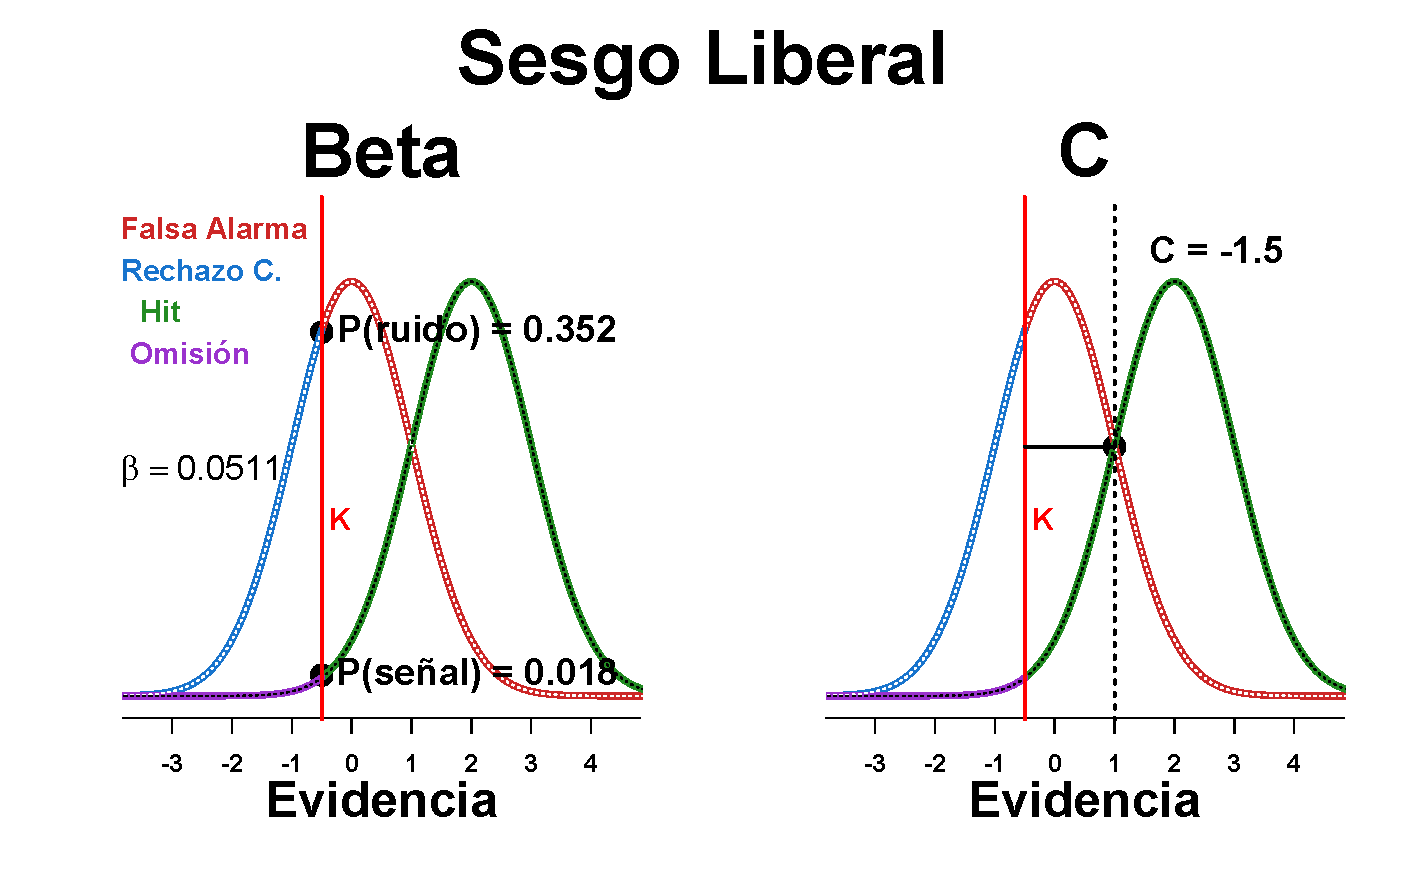
\includegraphics[width=0.75\textwidth]{Figures/Graficador_Sesgo_LiberalR}\\
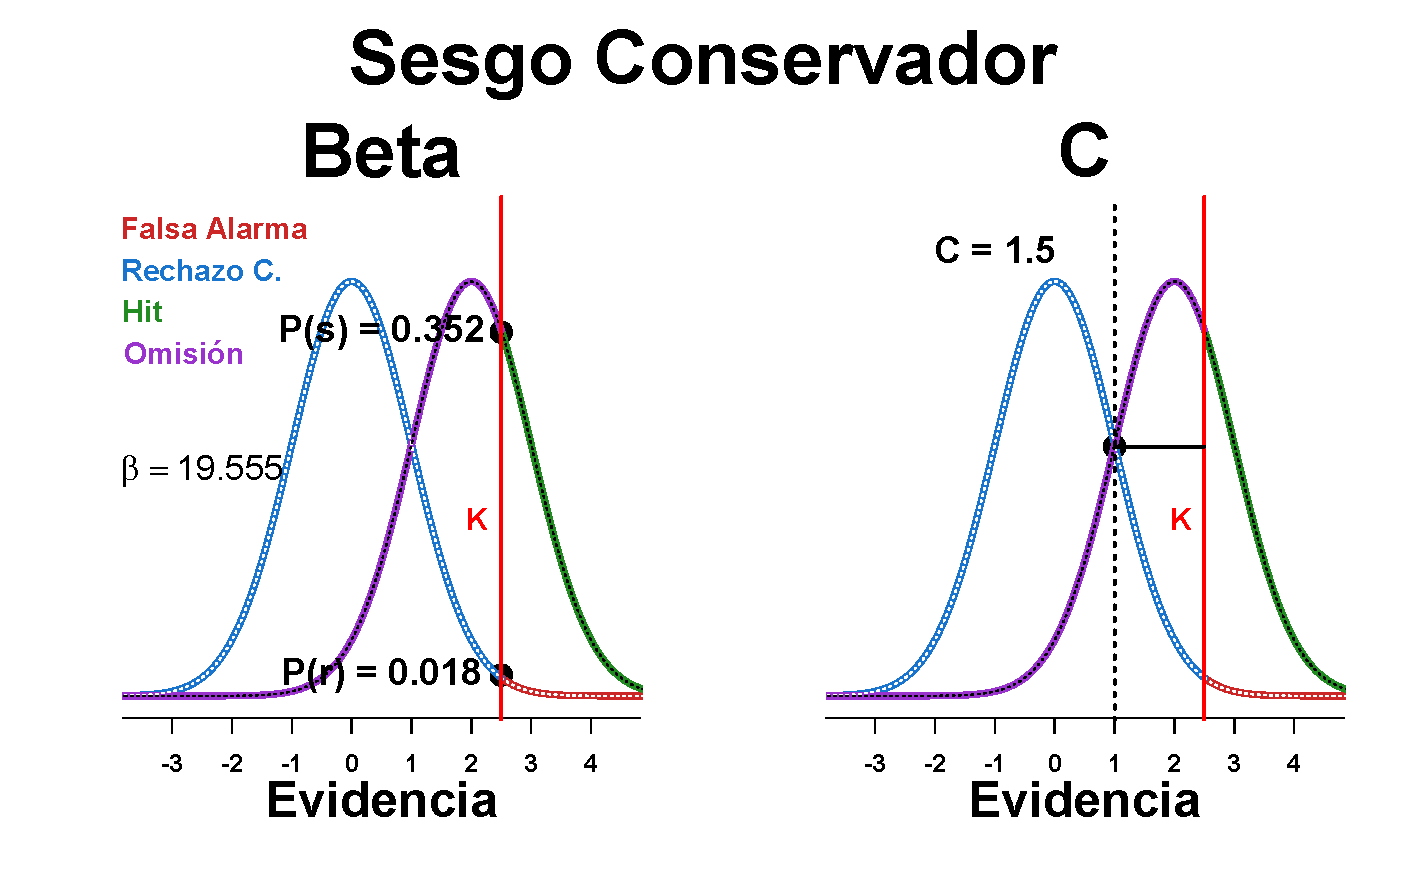
\includegraphics[width=0.75\textwidth]{Figures/Graficador_Sesgo_ConservadorR}\\
\decoRule
\caption[Estimación paramétrica: Sesgos $\beta$ y $c$]{Se ilustran los parámetros de sesgo $\beta$ (izquierda) y $C$ (derecha), en casos donde el sesgo del sistema es liberal (panel superior) o conservador (panel inferior).}
\label{fig:Graf_Sesgo}
\end{figure}

\end{itemize}

Para una exposición más detallada e interactiva de los parámetros descritos hasta ahora, se pueden consultar los graficadores y Apps en línea desarrollados por la autora de la presente tesis y otros colaboradores del Lab 25, como parte de un proyecto PAPIME (\citeyear{PAPIME}). Estos materiales se encuentran disponibles en \href{http://www.bouzaslab25.com/LabVirtual25/}{bouzaslab25.com/LabVirtual25}, un sitio web diseñado por la autora de esta tesis para los estudiantes de los cursos impartidos por el Dr. Arturo Bouzas.\\
%----------------------------------------------------------------

\subsection{Curvas ROC}

Además de permitir la descripción e interpretación del desempeño observado en tareas de detección a partir de la estimación de los parámetros descritos, los datos obtenidos en sesiones experimentales pueden ser utilizados para una evaluación más completa de la precisión con que el sistema podría responder a la misma tarea usando distintos criterio de elección. Las curvas ROC (identificadas así por su nombre en inglés: Receiver-Operating Characteristic Curve) describen la relación entre las tasas de Hits y Falsas Alarmas a obtener en tareas de detección con un valor partiular de $d'$, por cada localización posible del criterio sobre el eje de evidencia (McNicol \citeyear{McNicol2}; Egan, Schulman y Greenberg, \citeyear{Egan1959}; Swets, \citeyear{Swets1973}).\\

La Figura~\ref{fig:Graf_ROC} ilustra la construcción de curvas ROC a partir de las tasas de ejecución registradas en tareas de detección. En las figuras izquierdas se presentan un par de representaciones arbitrarias de tareas con distintos niveles de $d'$ y criterios en $k$. Las figuras del lado derecho, señalan con un punto las coordenadas que corresponden a las tasas de Falsas Alarmas (eje x) y Hits (eje y) obtenidas y, de acuerdo con el valor de $d'$ estimado, la curva ROC que describe todos los posibles pares de Hits y Falsas Alarmas a observar con el uso de distintos criterios de elección. La idea central, es que por cada $d'$ se puede trazar una curva ROC que describa los resultados esperados para todos los valores posibles de $k$ (Tanner y Swets, \citeyear{Tanner1954}; Swets y cols.,  \citeyear{Swets1961}; Swets, \citeyear{Swets1973}; Stainslaw y Todorov, \citeyear{Stainslaw1999}).\\

\begin{figure}[p]
\centering
%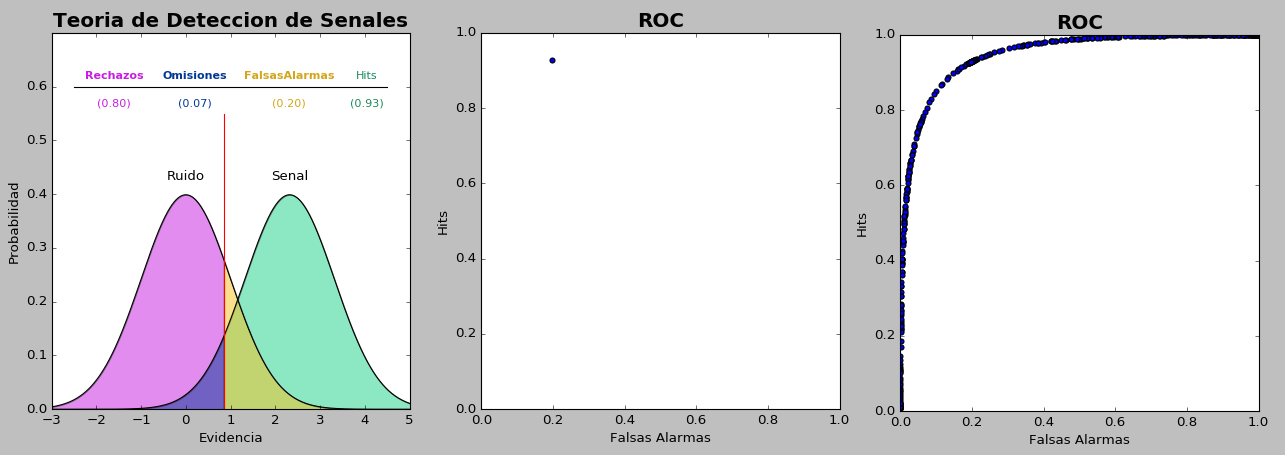
\includegraphics[width=0.90\textwidth]{Figures/Graficador_ROC12}\\
%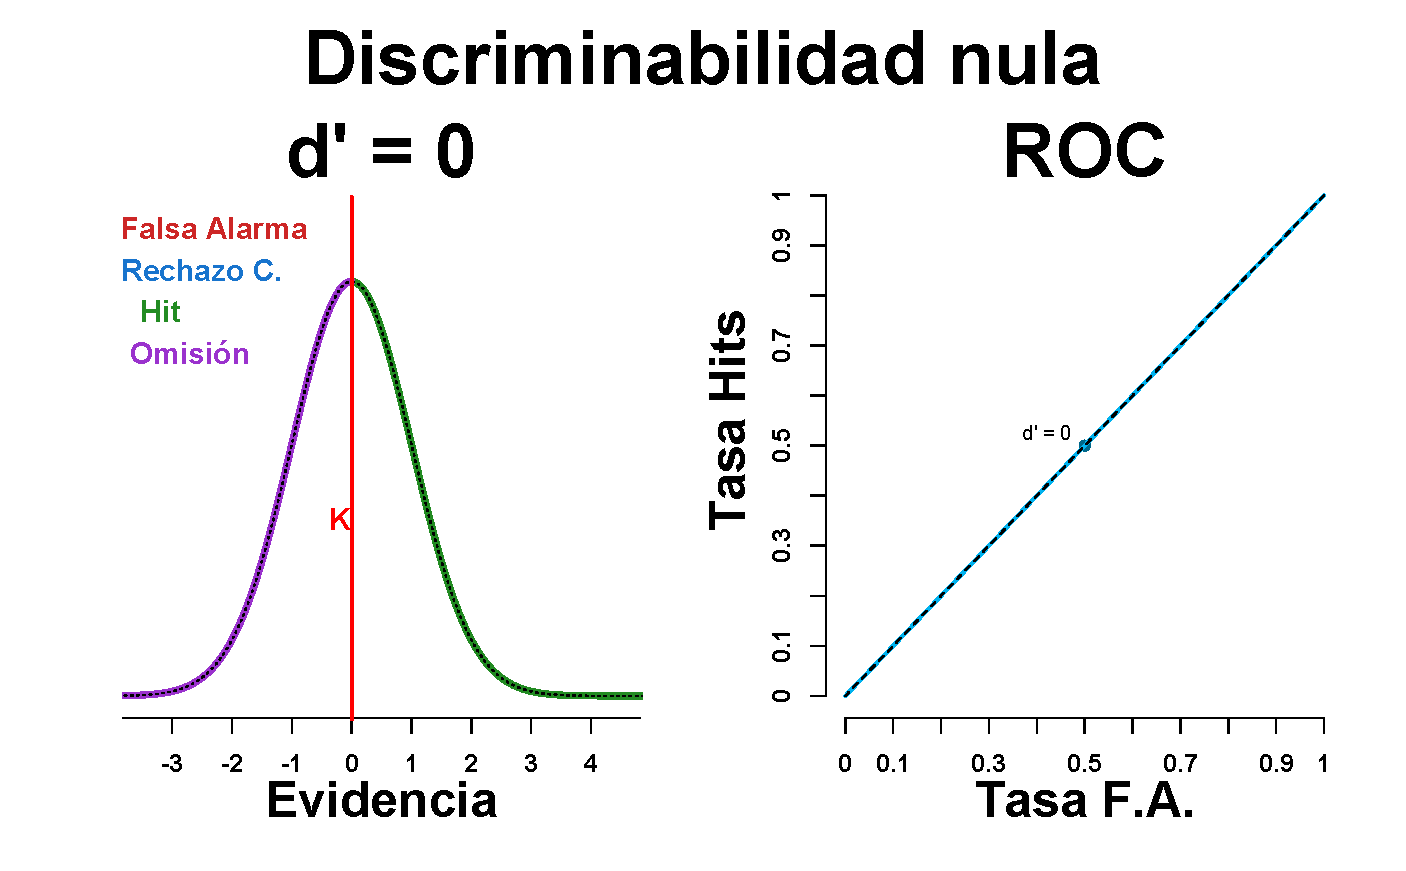
\includegraphics[width=0.9\textwidth]{Figures/ROC_1}\\
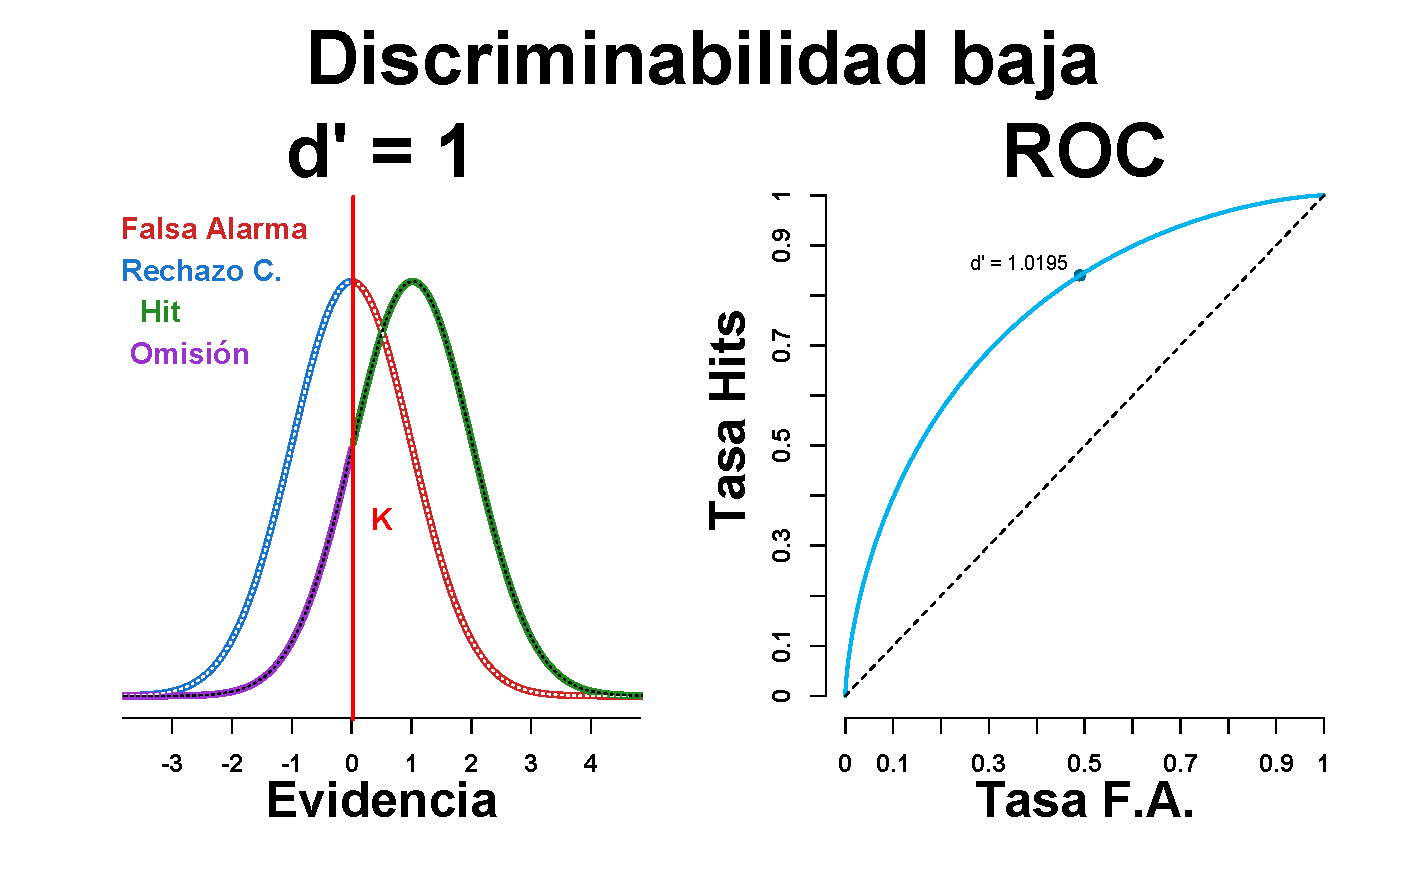
\includegraphics[width=0.8\textwidth]{Figures/ROC_2} \\
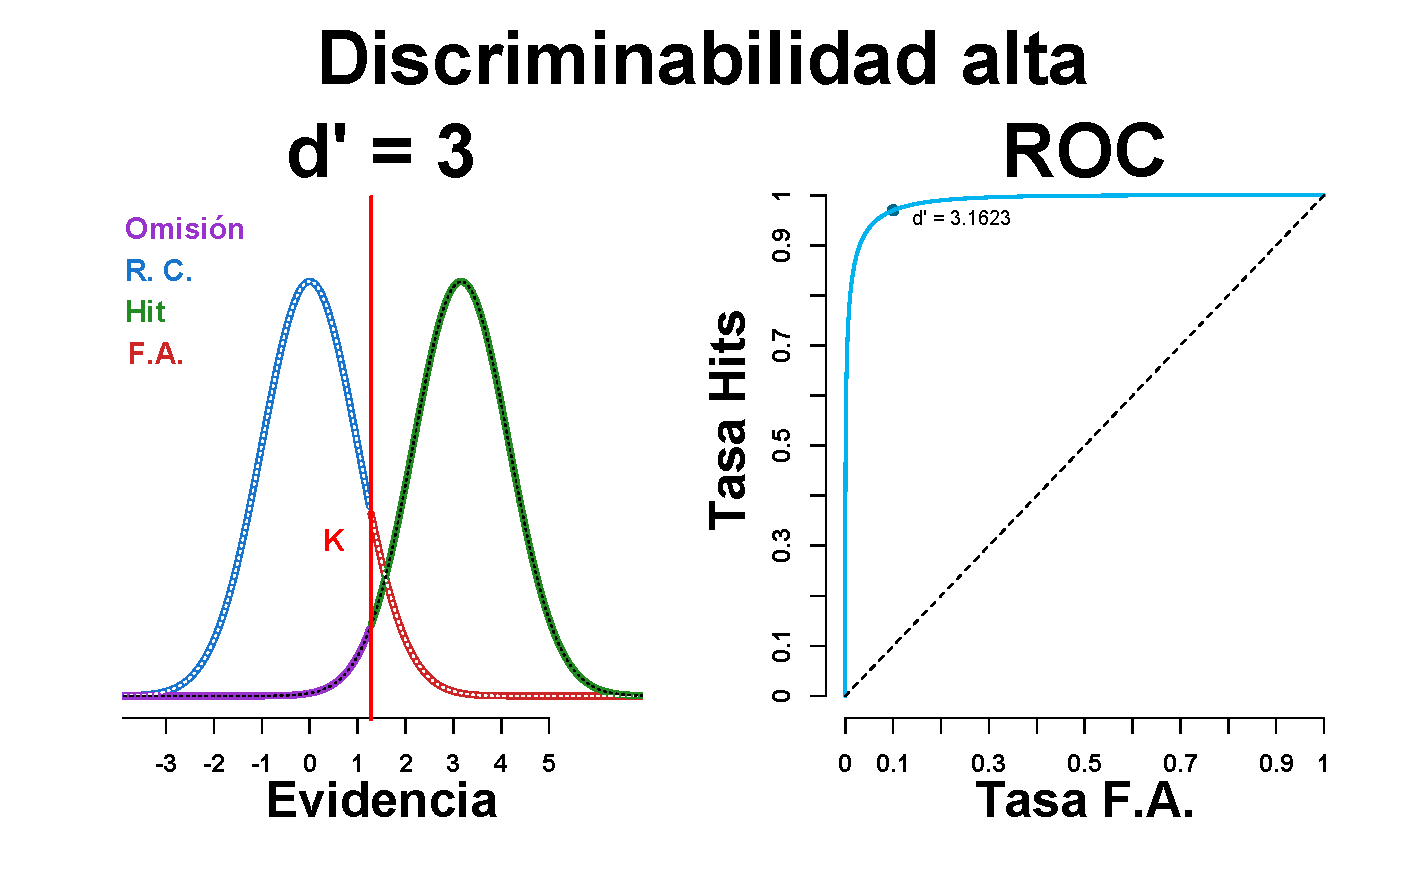
\includegraphics[width=0.8\textwidth]{Figures/ROC_3}\\
\decoRule
\caption[Trazo de curvas ROC]{Ilustración del trazo de curvas ROC en dos escenarios con distinto nivel de $d'$. Los puntos marcados en las curvas ROC (figuras derechas) corresponden con la relación Tasa de Hits y Falsas Alarmas observadas dada la localización del criterio (figuras izquierdas). Las líneas contínuas azules en las curvas ROC representan los posibles pares a observar entre las tasas de Hits y Falsas Alarmas, dada la $d'$ computada, por cada valor que pueda ocupar el criterio.}
\label{fig:Graf_ROC}
\end{figure}

%Bajo el supuesto de que lo único sobre lo que el sistema detector tiene injerencia es sobre el criterio de elección a usar para emitir sus juicios de detección, y que la discriminabilidad -al ser una cualidad inherente a los estímulos comprometidos en la tarea (ya sea por la variabilidad en su presentación o percepción)- es constante y ajena a este, \\

El área bajo la curva ROC (AUC, por sus siglas en ingles: Area Under the Curve) representa una forma precisa y completa de evaluar la sensibilidad del sistema detector ante la tarea estudiada (Centor y Schwartz, \citeyear{Centor1985}; Stainslaw y Todorov, \citeyear{Stainslaw1999}; McNicol, \citeyear{McNicol5}). Nótese que se habla de \textit{Sensibilidad} y no de \textit{Discriminabilidad} porque, aunque ambos conceptos refieren a qué tan fácil es para el sistema distinguir entre la señal y el ruido y se relacionan directamente con la distancia que existe entre sus distribuciones, la primera apela a la precisión con que el sistema detector puede responder a la tarea -utilizando distintas estrategias o reglas de elección- y la segunda, a una cualidad inherente a los estímulos (Swets, \citeyear{Swets1973}).\\

Como se mencionó anteriormente, en general se sabe que mientras más grande sea $d'$, existe una menor incertidumbre en la tarea de detección evaluada. Sin embargo, es complicado interpretar dicho valor en términos de qué tan \textit{buena} es la discriminabilidad. Es decir, parece poco claro qué tanto tendría que alejarse $d'$ de $0$ para afirmar que la Señal es discriminable del Ruido. Para ello, el cálculo del AUC proporciona información valiosa para la evaluación de la precisión con que el sistema puede responder a la tarea evaluada (Stainslaw y Todorov, \citeyear{Stainslaw1999}).\\ 

Cuando los estímulos con Señal son indistinguibles de los estímulos con Ruido ($d' = 0$), la curva ROC resultante se ve como una función de identidad. Esto implica que al emitir un juicio de detección afirmativo, existe la misma probabilidad de que este resulte en un Hit o una Falsa Alarma, con un AUC de 0.5 (la mitad del área total cae por debajo de la curva). Es decir, que mientras mayor sea el valor de $d'$, la curva ROC resultante se alejará más de la función identidad y su AUC será cada vez más cercano a 1.0. En general, el AUC puede tomar valores entre 0.5 -un sistema que no distingue en lo absoluto entre la Señal y el Ruido- y 1.0 -distinción perfecta entre los mismos- (Swets, \citeyear{Swets1973}; Stainslaw y Todorov, \citeyear{Stainslaw1999}; McNicol, \citeyear{McNicol5}).\\

Las curvas ROC pueden ser trazadas -en teoría- a partir de un solo conjunto de tasas de ejecución (Pollsvk y Norman, \citeyear{Pollack1964a}; Pollack, Norman y Galanter, \citeyear{Pollack1964b}; McNicol, \citeyear{McNicol2}) mediante algoritmos que asumen que el desempeño observado por parte del participante no puede \textit{mejorar} o \textit{empeorar} (dado que la discriminabilidad no depende de su conducta), y que se limitan a computar las tasa de ejecución que se esperaría observar en cada ubicación posible del criterio. Sin embargo, también pueden trazarse varios puntos para guiar el trazo de la curva ROC a partir de datos obtenidos en tareas donde experimentalmente se induzca el uso de distintos criterios de elección, obteniendo varios pares de tasas de Hits y Falsas Alarmas (Egan y cols., \citeyear{Egan1959}; Swets y cols., \citeyear{Swets1961}; Swets, \citeyear{Swets1986}). Los procedimientos mediante los cuales esto se lleva a cabo se discuten en la sección siguiente.\\

Al contar con datos obtenidos experimentalmente sobre el uso de distintos criterios de elección para responder a una misma tarea de detección, se puede trazar un tipo especial de curva ROC que permite explorar las características de las distribuciones de ruido y señal subyacentes. Para ello, en vez de graficar la relación entre las tasas observadas de Falsas Alarmas y Hits, éstas se transforman en Puntajes Z para obtener lo que se conoce como una curva \textbf{z-ROC} que permite evaluar tres grandes factores (Ratcliff y cols., \citeyear{Ratcliff1992}):\\♠

\begin{itemize}
\item Si la curva z-ROC trazada es una línea recta, se acepta el supuesto de que las distribuciones de Ruido y Señal son normales.
\item La pendiente de la curva z-ROC permite conocer la razón entre las desviaciones estándar de las distribuciones de Ruido y Señal, evaluando así el supuesto de las varianzas iguales.
\item El intercepto de la curva z-ROC proporciona información sobre la distancia entre las distribuciones (un aproximado de $d'$).
\end{itemize}


%----------------------------------------------------------------

\subsection{Tareas de detección}

Para la interpretación y evaluación de tareas de detección, existen tres grandes protocolos empleados para obtener datos susceptibles de ser analizados bajo el marco de la SDT (McNicol, \citeyear{McNicol2}; Stainslaw y Todorov, \citeyear{Stainslaw1999}):\\

\begin{itemize}
\item \underline{Tareas de detección binaria}\\

La forma más sencilla y estándar de presentar una tarea de detección es con un procedimiento que únicamente solicite a los participantes la emisión de juicios binarios de detección (\textit{'Sí, la señal está'} o \textit{'No, no está'}). Dicho protocolo se identifica en la literatura con el nombre de \textbf{tareas de detección binaria} o \textbf{tareas Sí/No} (McNicol, \citeyear{McNicol2}).\\

Las tareas Sí/No realizadas en el laboratorio consisten en la presentación aleatoria de una serie de ensayos (N) compuesta por ensayos que contienen la señal (S) y ensayos con sólo ruido (R). En cada ensayo, la única respuesta que los participantes deben registrar es si la señal estuvo presente o no.\\

Típicamente, la cantidad de ensayos S y R presentados durante la tarea es la misma. Esto es recomendable por dos grandes razones: 1) Garantiza que las cuatro tasas de ejecución observadas sean igual de representativas del desempeño del participante, quien habría tenido el mismo número de oportunidades de cometer cada tipo de acierto y error, y 2) Evita que los participantes desarrollen un sesgo a favor de una respuesta particular dependiendo cuál sea el tipo de ensayo que más se le presente (Nevin, \citeyear{Nevin1969}; Wickens, \citeyear{Wickens1}).\\

Por cada tarea Sí/No conducida, se obtiene un conjunto de tasas de ejecución que permiten trazar uno solo de los puntos que componen la curva ROC que describe la sensibilidad del sistema evaluado. Así que, para obtener más datos con los cuales trazar la curva (más conjuntos de tasas de ejecución), tendría que correrse la misma tarea en repetidas ocasiones, con los mismos estímulos y en los mismos participantes, pero incitando el uso de distintos criterios de elección en cada ocasión. Esto se puede hacer de manera explícita (solicitándole al participante que sea más o menos estricto en la emisión de sus respuestas), o implícita (por ejemplo, presentando la tarea con distintas matrices de pago que lleven al participante a evitar un cierto tipo de error, o a buscar cierto tipo de acierto) (Wickens, \citeyear{Wickens1}; McNicol \citeyear{McNicol2}.\\

Un problema evidente con el trazo de curvas ROC a partir de los datos obtenidos en tareas de detección binarias repetidas es que requiere un número considerable de repeticiones, todas compuestas por el mismo número de ensayos. Exponer a un mismo participante a la misma tarea varias veces trae consigo el riesgo de que su desempeño se vea afectado por la fatiga o el aprendizaje. Si este fuera el caso, los datos obtenidos no sólo serían reflejo de cambios en el criterio usado para responder a la tarea, sino que incluso podría haberse alterado la discriminabilidad de la misma (el aprendizaje puede hacer que los participantes se vuelvan mejores distinguiendo entre la Señal y el Ruido, y la fatiga, tener el efecto opuesto). Esto representa un problema porque entonces, la curva ROC trazada no representaría la sensibilidad del sistema evaluado ante \textit{una misma} tarea, pues se estaría violando el supuesto fundamental de que la discriminabilidad es constante (McNicol, \citeyear{McNicol2}).\\

\item \underline{Tareas con Escala de Confianza}\\

Una segundo protocolo para la presentación de tareas de detección -que puede entenderse como una extensión de las tareas Sí/No- es solicitando a los participantes que valoren y asignen un puntaje a la certeza que tienen sobre la pertenencia de cada estímulo evaluado a las categorías Señal o Ruido, de acuerdo con una \textbf{Escala de Confianza}.\\

En términos del procedimiento, las tareas de detección binarias y con Escala de Confianza son idénticas: se muestra a los participantes una serie de ensayos (N) dentro de la cual se presentan de manera aleatoria ensayos con la señal (S) y ensayos con sólo Ruido (R), solicitándoles que registren una respuesta al término de cada ensayo. La diferencia entre ambos protocolos consiste en el tipo de respuesta solicitada y, en consecuencia, la cantidad de información que se obtiene sobre la sensibilidad del sistema. En las tareas Sí/No los participantes emiten una de dos posibles respuestas mutuamente excluyentes; en tareas con Escala de Confianza, se asigna un puntaje dentro de una Escala con cierta cantidad de opciones de respuesta (Stainslaw y Todorov, \citeyear{Stainslaw1999}).\\

\begin{figure}[p]
\centering
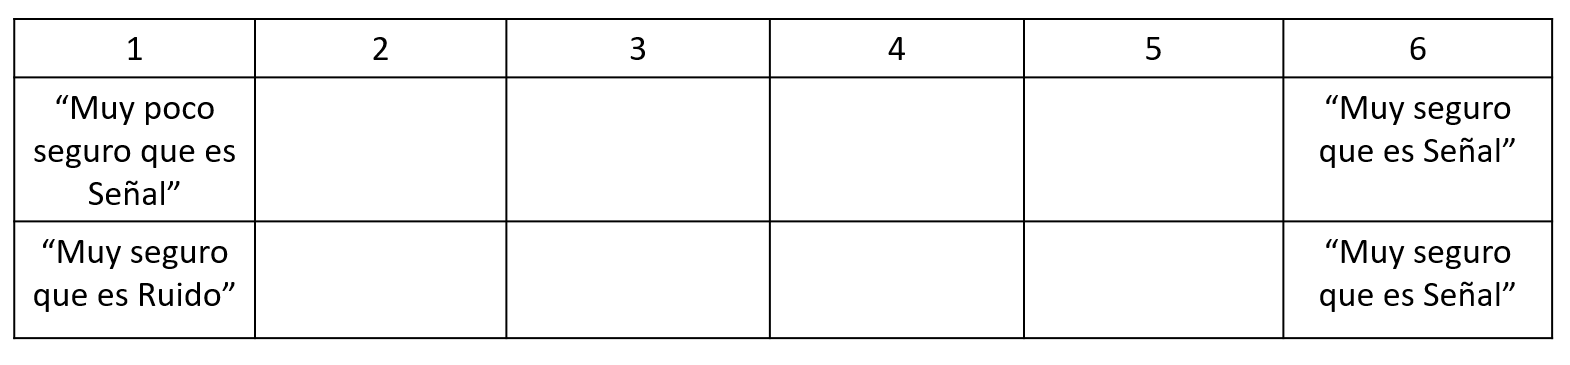
\includegraphics[width=0.9\textwidth]{Figures/Puntajes_Criterios}\\
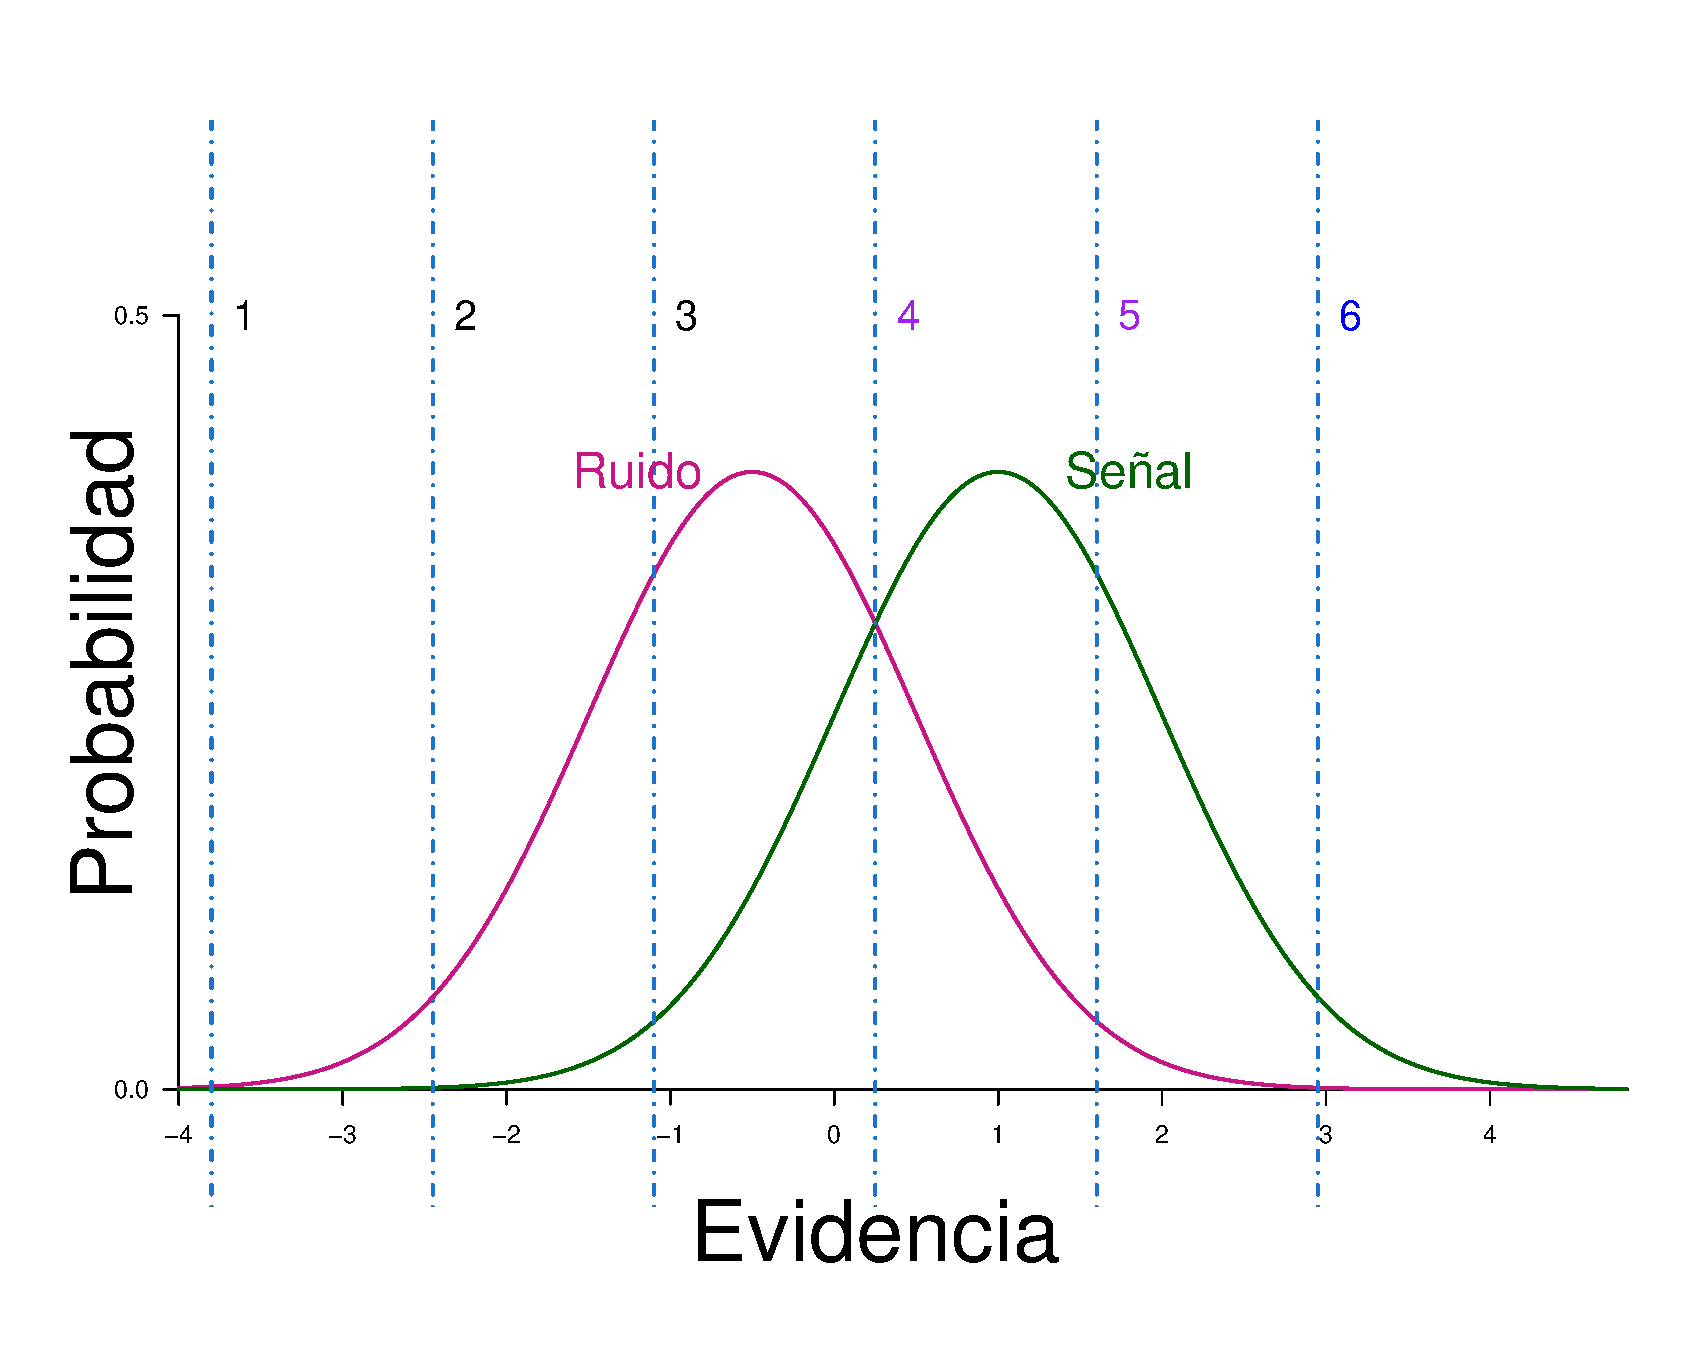
\includegraphics[width=0.8\textwidth]{Figures/ConfidenceRating}\\
\decoRule
\caption[Tareas de detección con Escala de Confianza y su interpretación]{Representación gráfica de la interpretación de las tareas de detección con Escala de Confianza bajo el marco de la SDT. En la parte superior se presenta una Escala de Confianza de seis elementos con dos posibles sentidos: unidireccional (el puntaje refleja la confianza en una sola respuesta) o bidireccional (el puntaje distingue entre la confianza en cada respuesta). La gráfica inferior ilustra la idea de que para decidir cuándo emitir cada puntaje, el sistema fija múltiples sub-criterios sobre el eje de evidencia.}
\label{fig:Conf_Rat}
\end{figure}

Existen varias formas en que puede presentarse la Escala de Confianza (McNicol, \citeyear{McNicol2}). Por ejemplo, una de ellas podría ser solicitando que se responda de acuerdo a la confianza que se tendría en asignar cada estímulo evaluado a la categoria Señal (donde los valores más altos se asignarían a los estímulos que se encuentren más hacia la derecha en el eje de evidencia y los valores bajos, a los estímulos con Ruido, a la izquierda). Por otro lado, una segunda forma sería distinguiendo entre la certeza que se tiene sobre la pertenencia de cada estímulo evaluado al conjunto de las señales o el ruido, (los valores más altos indicarían confianza en que se trate de una Señal y los valores más bajos, de que se trate de Ruido). Ambas formas de presentar la Escala proporcionan -en teoría- la misma información, tal y como se sugiere en el panel superior de la Figura~\ref{fig:Conf_Rat}. En general, la elección de una u otra depende del experimentador.\\

Los puntajes de confianza registrados son interpretados asumiendo que los participantes fijan un criterio por cada opción de respuesta incluida en la Escala de Confianza. De esta forma, el puntaje emitido en cada ensayo está determinado por el último criterio de elección rebasado por la evidencia evaluada (McNicol, \citeyear{McNicol2}). La Figura~\ref{fig:Conf_Rat} ilustra esta idea: en la parte superior se presenta una Escala de Confianza de 6 elementos (se ejemplifican las dos formas -previamente expuestas- en que puede ser presentada), y en la parte inferior, la representación gráfica de su interpretación bajo el modelo de detección de señales.\\

El protocolo de Escala de Confianza permite recabar información sobre el uso de múltiples criterios de elección -tantos como opciones de respuesta se incluyan en la Escala- en una tarea de detección particular con un solo experimento, manteniendo constante la discriminabilidad. Por ello, el uso de Escala de Confianzas con $n$ opciones de respuesta, representa una forma sencilla y directa de obtener datos suficientes para trazar $n - 1$ puntos en una curva ROC y poder evaluar con mayor certidumbre la sensibilidad del sistema (Stainslaw y Todorov, \citeyear{Stainslaw1999}; McNicol, \citeyear{McNicol2, McNicol5}).\\ 

Idealmente, se espera que el participante utilice todas las opciones de respuesta incluídas en la Escala de Confianza. Esto se puede conseguir de manera explícita o implícita, solicitando a los participantes que lo hagan así, o bien, modificando el número de puntajes incluídos en la Escala. En general, se recomienda que la Escala esté compuesta por un número par de opciones de respuestas que oscile entre 4 y 10 (McNicol, \citeyear{McNicol2, McNicol5}). Esto con el fin de evitar que los participantes elijan la opción intermedia cuando se sientan inseguros sobre su respuesta.\\

\item \underline{Tarea de Elección forzada}\\

Existe un tercer protocolo bajo el cual se presentan las tareas de detección, identificado como \textbf{tareas de Elección forzada entre $m$ alternativas}, donde se presentan simultáneamente $m - 1$ estímulos que contienen sólo ruido y $1$ con señal, y la tarea del participante consiste en identificar la Señal dentro del conjunto de estímulos que se le presentan (Stainslaw y Todorov, \citeyear{Stainslaw1999}). En general, se asume que cada estímulo presentado contiene cierto valor de evidencia -cierta ubicación en el eje sobre el cual se despliegan las distribuciones- que el participante compara para elegir aquel que tenga un valor mayor -de acuerdo con el supuesto que establece que, en general, los valores de la distribución Señal caen por encima del Ruido- (McNicol, \citeyear{McNicol2}).\\

%Dada la relación que representan, el área bajo la curva ROC trazada con un protocolo de preguntas binarias o con Escala de Confianza puede interpretarse como la proporción de veces que el participante cuyo desempeño se describe, podría identificar correctamente la Señal, si esta fuera presentada simultáneamente junto con el Ruido. A su vez, la proporción de respuestas correctas obtenidas a lo largo de una tarea de Elección forzada proporciona una medida de la sensibilidad del sistema, independiente del sesgo del sistema. Dicha medida -al igual que el AUC-, tendría que variar entre el azar ($\frac{1}{m}$) y el desempeño perfecto ($1.0$), \citep{Stainslaw1999}.\\
\end{itemize}


















\section{Teoría de Detección de Señales en Memoria}

La Teoría de Detección de Señales ha sido ampliamente utilizada en distintas áreas de la Psicología Experimental tanto como marco de referencia para la descripción de diversas situaciones de detección, como herramienta para el análisis de datos obtenidos en dichas tareas. Una de estas áreas refiere al estudio de la Memoria, donde los supuestos y conceptos desarrollados en la SDT han sido aplicados para explicar el funcionamiento del aprendizaje humano, la retención, el olvido y el reconocimiento de estímulos (Murdock, \citeyear{Murdock1965}; Bernbach, \citeyear{Bernbach1967}; Lockhart y Murdock, \citeyear{Lockhart1970}; Banks, \citeyear{Banks1970}; WHite y Wixted, \citeyear{WHite1999}).\\

%Al estudiar las tareas presentadas en estudios de memoria como instancias de un problema de detección, los resultados obtenidos pueden clasificarse dentro de las mismas categorías presentadas anteriormente en la matriz de la Figura~\ref{fig:Mat_Output}), permitiendo así que las tasas de Hits y Falsas Alarmas registradassean uilizadas para trazar curvas ROC (Egan, \citeyear{Egan1958}; Zandt, \citeyear{VanZ2000}), con frecuencia identificadas como curvas MOC (por sus siglas en inglés \textit{Memory Operant Curve}), (Norman y Wickelgreen, \citeyear{Norman1965}; Kintsch y Carlson, \citeyear{KintschCarlson1967}).\\

La aplicación de la SDT al estudio de la memoria ha impactado en el desarrollo de este útlimo en términos de cuatro grandes ejes (Banks, \citeyear{Banks1970}), que son:\\

\begin{enumerate}
\item La noción de la \textit{Fuerza de Memoria}.\\

Aceptar la SDT como marco para describir el funcionamiento de los distintos mecanismos estudiados en Memoria implica asumir que la \textit{evidencia} con base en la cual se emiten las respuestas ensayo a ensayo son valores ($x$) dentro de un eje contínuo sobre el cual se despliegan las distribuciones de Ruido (los estímulos distractores) y Señal (estímulos definidos de acuerdo al procedimiento empleado). Los modelos de memoria que incorporan la SDT como base para el desarrollo de su marco explicativo, tienden a interpretar dicho valor $x$ como un reflejo de la \textit{fuerza de memoria}, o bien, un índice de qué tan \textit{relacionable} o \textit{familiar} resulta para el sistema cada estímulo evaluado (Ratcliff, Ching-FanSheu y Gronlund, \citeyear{Ratcliff1992}). Así pues, se interpreta el desempeño observado en los participantes como resultado de la interacción entre la \textit{fuerza de memoria} evaluada en cada ensayo y un proceso de decisión que determina si ésta es lo suficientemente grande para juzgar la pertenencia de cada estímulo a la categoría Señal.\\

%En términos de la exploración de este supuesto y sus implicaciones, resaltan los trabajos orientados a evaluar la naturaleza de dicha \textit{fuerza de memoria} (por ejemplo, si puede entenderse a partir de valores contínuos o discretos), y su interacción con los procesos propios de la Memoria (por ejemplo, el estudio, la retención y el olvido), (Bernbach, \citeyear{Bernbach1967}; Wickelgreen y Norman, \citeyear{Wickelgren1966}; Parks, \citeyear{Parks1966}).\\

\item La noción del Criterio de Elección como opuesta a los Umbrales de respuesta.\\

Una de las aportaciones más evidentes de la aplicación de los principios propuestos por la SDT al estudio de la Memoria es que permite entender los Falsos Positivos en términos de una confusión entre la fuerza de memoria producida por un estímulo distractor y la Señal (el área de sobrelape entre las distribuciones), y abandonar el supuesto de que cuando las señales a detectar están ausentes, los participantes responden a la tarea de manera aleatoria. Con ello, se abandona la noción originada en la Teoría del Umbral de que existe tal cosa como un \textit{umbral de memoria} que debe ser rebasado para que el sistema sea capaz de identificar la pertenencia de los estímulos a una u otra categoria (Murdock, \citeyear{Murdock1982}; Gillund y Shiffrin, \citeyear{Gillund1984}; Yonelinas, Dobbins, Szymanski Dhaliwal y King, \citeyear{Yonelinas1996}; Wixted, \citeyear{Wixted2007}). Con ello, tal y como ocurrió tras la incorporación de la SDT al estudio de la Percepción, los procesos de Memoria comienzan a ser concebidos como instancias de un proceso de decisión (Bernbach, \citeyear{Bernbach1967}).\\
 
\item La noción de que existen distribuciones subyacentes (y la definición de sus características).\\

Los datos obtenidos en experimentos de memoria donde se promueva el uso de diversos criterios de elección pueden utilizarse para construir curvas \textbf{MOC} (por sus siglas en inglés, Memory Operating Characteristic curve) que describan la precisión con que los participantes distinguen entre los estímulos con ruido y señal, (Kintsch, \citeyear{Kintsch1967}; Ratcliff y cols., \citeyear{Ratcliff1992}; Ratcliff, McKoon y Tindall, \citeyear{Ratcliff1994}). Así mismo, el trazo de curvas MOC a partir de las transformaciones a Puntajes Z de las tasas de Hits y Falsas Alarmas registradas (lo que serían las curvas z-MOC), ha permitido explorar la naturaleza de las distribuciones subyacentes (Ratcliff y cols., \citeyear{Ratcliff1992}), los hallazgos e implicaciones de este tipo de análisis se desarrollan más adelante.\\
\end{enumerate} 

\subsection{Memoria de Reconocimiento}

%Por mucho tiempo, los modelos desarrollados en Memoria estuvieron muy limitados en términos del espectro de tareas y fenómenos de los que permitían dar cuenta. No fue hasta que comenzaron a surgir los \textit{modelos globales de memoria}, que incorporaron los principios básicos de la SDT, que fue posible explicar una gama más amplia de tareas y mecanismos dentro del área. Estos modelos se distinguen principalmente por los supuestos que hacen sobre el tipo de distribuciones que capturan la variabilidad contenida en los estímulos con ruido y señal, y la forma en que se define la fuerza de memoria en la interacción entre los distintos sistemas de memoria y los estímulos (Murdock, \citeyear{Murdock1982}; Gillund y Shiffrin, \citeyear{Gillund1984}; Eich, \citeyear{Eich1985}). Cada uno de estos modelos ha sido desarrollado para dar cuenta de un sub-set específico de tareas y fenómenos (recuerdo, juicios de frecuencia, olvido y retención, entre otros), encontrando un punto de convergencia en el estudio de la Memoria de Reconocimiento (Parks, \citeyear{Parks1966}; Ratcliff y cols., \citeyear{Ratcliff1992}).\\

Los modelos que incorporan la SDT para dar cuenta de la Memoria de Reconocimiento aparecen como una alternativa a los modelos clásicos que adoptaban la idea de \textit{umbrales de respuesta} (Yonelinas y cols., \citeyear{Yonelinas1996}; Wixted, \citeyear{Wixted2007}). Bajo el marco de la SDT, las tareas de reconocimiento comienzan a ser convebidas como una instancia de tareas de detección, donde los participantes tienen que identificar elementos que ya se le habían mostrado en una fase previa de estudio (los \textit{estímulos viejos}: las señales) y rechazar aquellos que no (los \textit{estímulos nuevos}), (Bernbach, \citeyear{Bernbach1967}; Kintsch, \citeyear{Kintsch1967}). Bajo este esquema, la 'fuerza de memoria' refleja el grado en que un estímulo cualquiera es percibido como 'familiar' para el sistema y su comparación con el criterio de elección es lo que determina la respuesta dada por el mismo (\textit{'Sí, es un elemento antes visto'} o \textit{'No'}).\\ 

\begin{figure}[h]
\centering
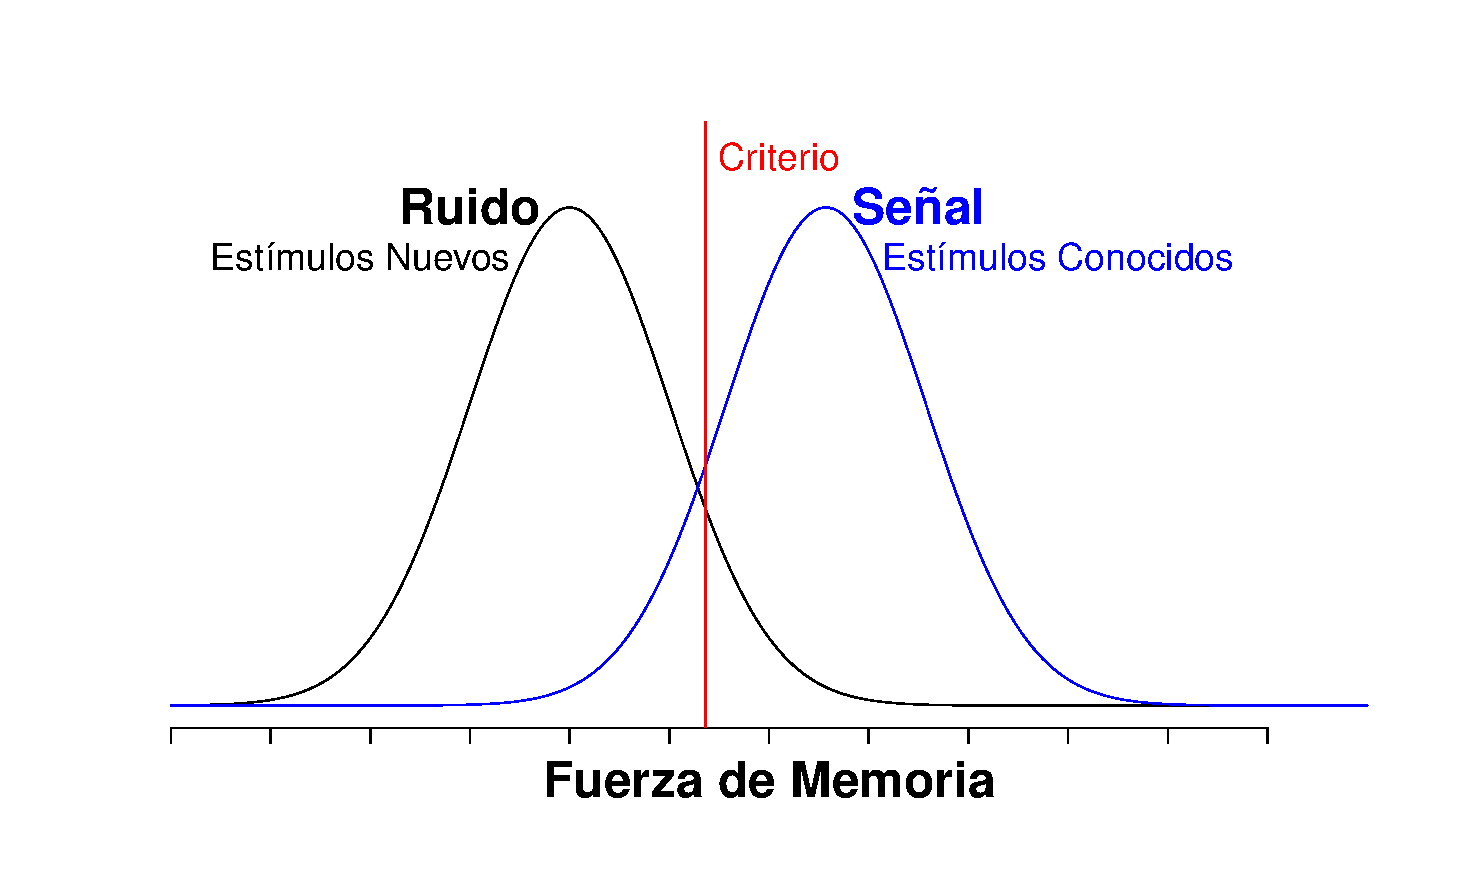
\includegraphics[width=0.8\textwidth]{Figures/RM_SDT_1} 
\caption[SDT aplicada a tareas de memoria de reconocimiento]{Representación gráfica de la aplicación de la SDT al estudio de tareas de memoria de reconocimiento}
\label{fig:RM_SDT_1}
\end{figure}

La Figura~\ref{fig:RM_SDT_1} ilustra la forma en que los supuestos y conceptos básicos de la SDT se aplican al contexto de la memoria de reconocimiento: Los estímulos ya conocidos (referidos como \textit{estímulos viejos}) constituyen la Señal y el Ruido lo componen estímulos nuevos que pueden ser confundidos con los viejos. El \textit{eje de evidencia} a lo largo del cual se despliegan las distribuciones se convierte en un \textit{eje de familiaridad}, que contiene distintos valores de 'fuerza de memoria' (siendo que los estímulos viejos tienen valores más altos de 'familiaridad' que los estímulos nuevos). Por último, se incorpora la idea de que la emisión de juicios de reconocimiento depende de la comparación entre la 'familiaridad' evaluada en cada ensayo y un criterio de elección fijado por el participante.\\

Las tareas de reconocimiento conducidas en el laboratorio suelen componerse de dos fases (Ratcliff y cols., \citeyear{Ratcliff1992}). En la primera (\textit{la fase de estudio}) se presenta a los participantes una serie de elementos para que los estudien de manera intencional (solcitándoles explícitamente que las estudien para su reconocimiento posterior) o incidental (planteándoles alguna tarea distractora que los obligue a interactuar con ellos) (Noldy, Stelmack y Campbell, \citeyear{Noldy1990}). En la segunda fase (la \textit{fase experimental} o \textit{de reconocimiento}) se presentan los mismos elementos incluidos en la primera fase, más una cantidad igual de elementos nunca antes presentados. La tarea de los participantes consiste en identificar cuáles de los elementos que se le presentan en la segunda fase son \textit{estímulos viejos}, previamente incluídos en la fase de estudio.\\

\begin{figure}[h]
\centering
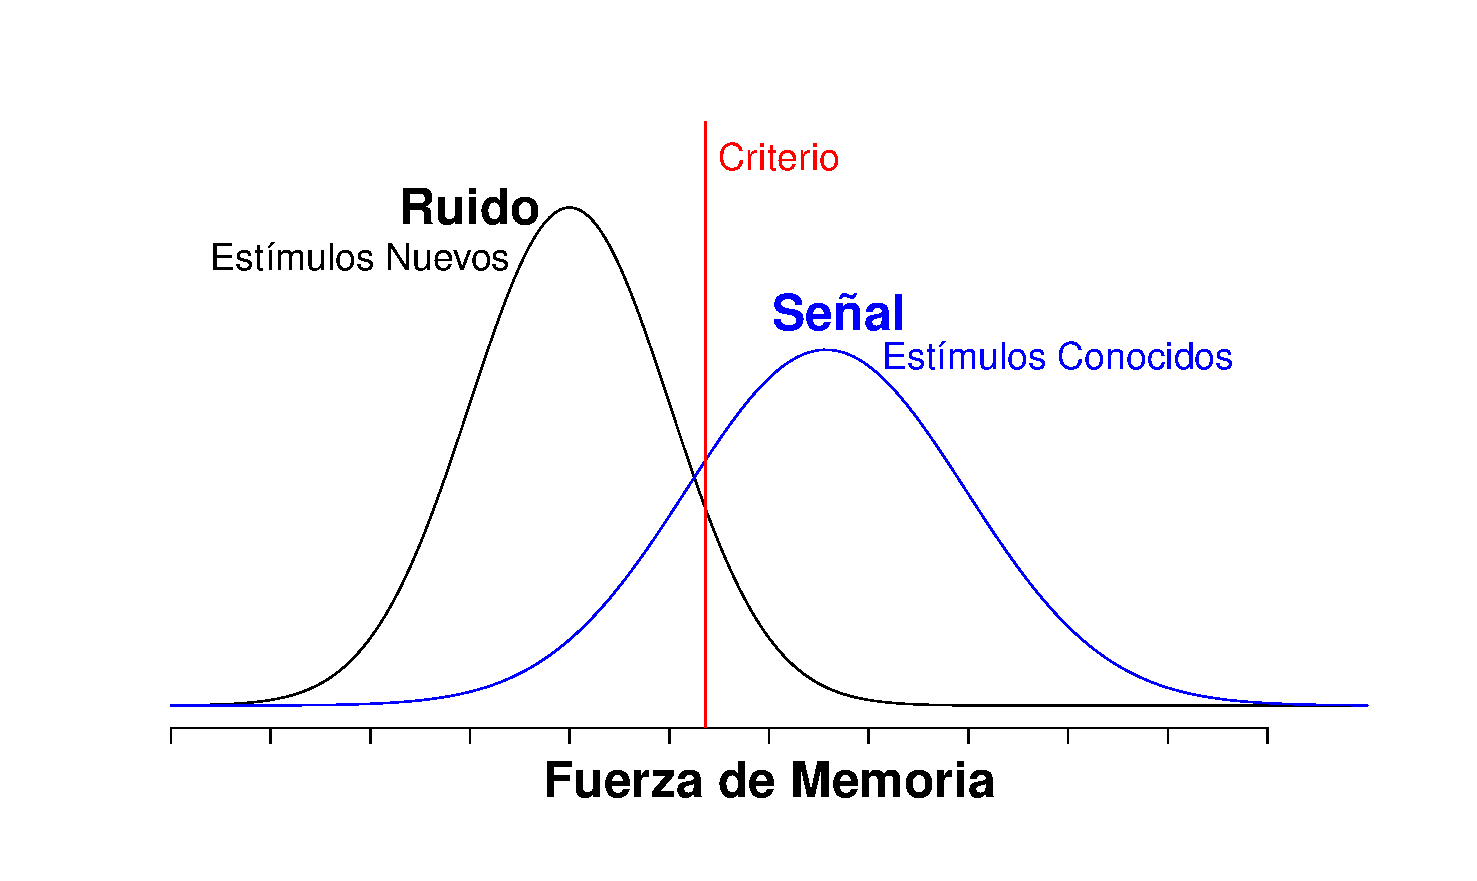
\includegraphics[width=0.80\textwidth]{Figures/RM_SDT_2} 
\caption[SDT en memoria de reconocimiento (varianzas desiguales)]{Representación gráfica del modelo de varianzas desiguales reportado en memoria de reconocimiento, al estudiarse bajo el marco de la SDT.}
\label{fig:RM_SDT_2}
\end{figure}

De acuerdo con las curvas z-ROC que se obtienen a partir de los datos obtenidos en estudios con tareas de reconocimiento, se ha concluído que el modelo basado en SDT que mejor describe la ejecución de los participantes es uno donde las distribuciones de Ruido y Señal son normales, siendo menor la varianza en la distribución de Ruido que en la distribución de Señal (Ratcliff y cols., \citeyear{ Ratcliff1992}, {Ratcliff1994}). Tal y como se ilustra en la Figura~\ref{fig:RM_SDT_2}, consistentemente se reporta que la razón entre las desviaciones estándar de la distribución de Ruido y Señal tiene valores cercanos a 0.8 (Wixted, \citeyear{Wixted2007}).\\






\section{El Efecto Espejo}

El 'Efecto Espejo' hace referencia a la interpretación de ciertos patrones de respuestas reportados consistentemente en estudios de memoria de reconocimiento donde el desempeño de los participantes es comparado a través de dos clases de estímulos que difieren en la precisión con que se sabe que sus elementos suelen reconocerse, bajo el marco de la SDT. Típicamente, dichas clases son referidas en la literatura como Clase A, con estímulos fácilmente reconocibles, y Clase B, con estímulos que se reconocen con mayor dificultad, (siendo que $d'(A) > d'(B)$), (Glanzer y Adams, \citeyear{Glanzer1990}). En estos estudios, se ha encontrado evidencia sólida de que las diferencias en la discriminabilidad de los estímulos Nuevos y Viejos de las clases A y B se mantienen en dos sentidos: en la identificacíón de los estímulos viejos como \textit{Viejos} (más Hits en A que en B) y en la identificación de los estímulos nuevos como \textit{Nuevos} (menos Falsas Alarmas en A que en B). Es decir, se ha encontrado evidencia que sugiere que las diferencias en $d'$ no sólo impactan en el número de Hits cometidos, sino también en la propoción observada de Falsas Alarmas (Glanzer, Adams, Iverson y Kim, \citeyear{Glanzer1993}).\\

Al interpretar las tasas de Hits y Falsas Alarmas registradas por cada clase bajo el marco de la SDT, se sugiere que existen cuatro distribuciones que subyacen a la tarea: dos distribuciones para los estímulos señal de cada clase y dos distribuciones de ruido. Y de acuerdo con los patrones de respuesta registrados, el orden en que se presentan las distribuciones de estímulos Viejos A y B es el inverso (el \textit{reflejo}) del orden en que se presentan las distribuciones de estímulos Nuevos respectivas (Glanzer y Adams, \citeyear{Glanzer1990}; DeCarlo, \citeyear{DeCarlo2007}). La representación gráfica de este orden (Nuevos(A), Nuevos(B), Viejos(B) y Viejos(A)), se presenta en la Figura~\ref{fig:Ejem_EfectoEspejo} e ilustra la razón por la cual se ha identificado dicho fenómeno con el nombre de Efecto Espejo.\\

\begin{figure}[h]
\centering
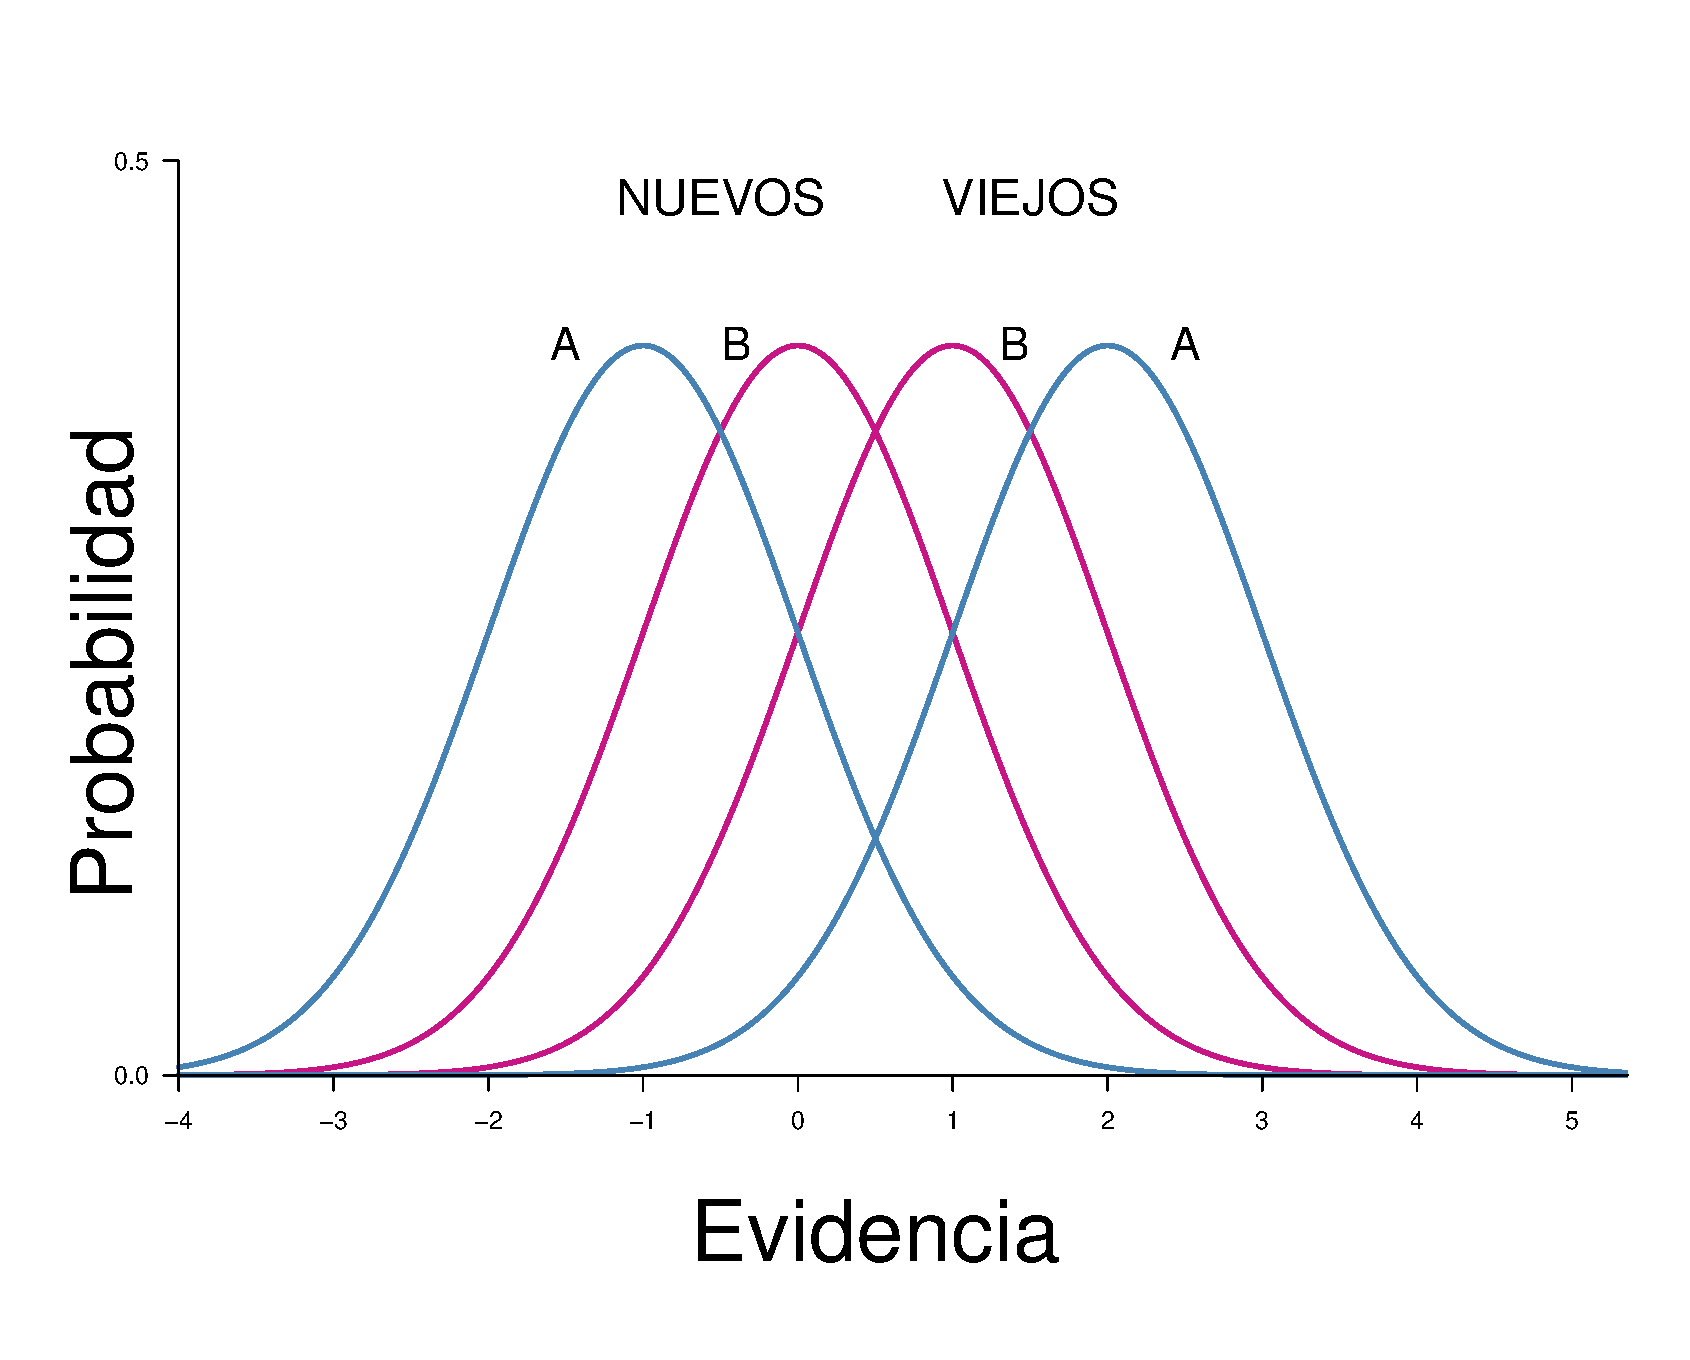
\includegraphics[width=0.7\textwidth]{Figures/EfectoEspejo}
\decoRule
\caption[Efecto Espejo: Las distribuciones de ruido y señal A y B se reflejan entre sí]{Representación gráfica de la ubicación de las distribuciones de ruido y señal (de las clases A y B) sobre el eje de evidencia, de acuerdo con los patrones de respuesta encontrados en tareas memoria de reconocimiento, identificados como Efecto Espejo.}
\label{fig:Ejem_EfectoEspejo}
\end{figure}

La evidencia a favor del Efecto Espejo en experimentos de memoria de reconocimiento se reporta a lo largo de una amplia variedad de clases de estímulos y protocolos de tareas de detección (Preguntas Sí/No; Escala de Confianza y Elección Forzada de dos alternativas), (Glanzer y Adams, \citeyear{Glanzer1990}), siempre y cuando se cumplan las siguientes condiciones:\\

\begin{itemize}
\item Existen al menos dos clases de estímulos A y B entre las cuales se compara el desempeño de los participantes. A y B difieren en su nivel de discriminabilidad: la clase A se caracteriza porque sus elementos se reconocen con mayor facilidad que los estímulos contenidos en B.\\

\item Los estímulos que componen las clases A y B se presentan de manera simultánea y aleatoria, tanto en la fase de estudio como en la de reconocimiento, sin que los participantes tengan forma de saber que se le está presentando más de un tipo de estímulo o que su desempeño se va a separar y comparar entre ambos. Esto se procura por dos razones: 1) permite asumir que los participantes están respondiendo con base en un sólo criterio de elección y 2) se controla que la forma en que las distribuciones subyacentes se escalan sea la misma (DeCarlo, \citeyear{DeCarlo2007}).\\
\end{itemize}

La separación que se observa en la Figura~\ref{fig:Ejem_EfectoEspejo} entre las distribuciones de estímulos Viejos A y B tiene sentido, ya que se espera que exista una mayor distancia entre la distribución Señal con la $d'$ más grande (Viejos(A)) y el ruido. Sin embargo, no hay razón para esperar que dicha diferencia se \textit{refleje} en dos distribuciones de estímulos Nuevos para las clases A y B, pues en el contexto de la memoria de reconocimiento no hay cómo explicar que el desempeño de los participantes difiera entre estímulos que sólo contienen ruido, ya que se trata de estímulos que no han sido mostrado previamente. En otras palabras, no parece haber forma de justificar las discrepancias reportadas entre las tasas de Falsas Alarmas registradas por cada clase, puesto que los estímulos A y B deberían ser igualmente \textit{familiares} en su primera exposición (Glanzer y cols., \citeyear{Glanzer1993}).\\

\subsection{Evidencia recolectada}

Como se mencionó previamente, la evidencia del Efecto Espejo en tareas de memoria de reconocimiento ha sido reportada a lo largo de distintos protocolos experimentales (Glanzer y Adams, \citeyear{Glanzer1990}; Glanzer y cols., \citeyear{Glanzer1993}). Los patrones de respuesta identificados en tareas Sí/No y con Escala de Confianza, así como su relación con la representación gráfica del Efecto Espejo (ver Figura~\ref{fig:Ejem_EfectoEspejo}), se exponen en detalle a continuación.\\

\begin{itemize}
\item \underline{Efecto Espejo en Tareas Sí/No}\\

En el caso de tareas Sí/No donde se presenta a los participantes aleatoriamente estímulos Nuevos y Viejos de las clases A y B para que indiquen si les reconocen como parte de la fase de estudio (\textit{'Sí, es un estímulo Viejo'}), o no (\textit{'No, es un estímulo Nuevo'}), se reporta el siguiente patrón de respuestas:

\begin{center}
$p[Si(NuevoA)] < p[Si(NuevoB)] < p[Si(ViejoB)] < p[Si(ViejoA)]$\\
donde $p[Si]$ es la proporción de juicios de reconocimiento afirmativos emitidos, (Glanzer, Adams, Kim e Iverson, \citeyear{Glanzer1993}).\\
\end{center}

De acuerdo con la correspondencia entre el tipo de estímulo presentado y los juicios afirmativos emitidos, esta misma relación puede definirse en términos de Hits y Falsas Alarmas:

\begin{center}
$FA(A) < FA(B) < H(B) < H(A)$\\
donde $FA$ y $H$ señalan las tasas de Hits y Falsas Alarmas observadas en cada clase (Glanzer y cols., \citeyear{Glanzer1993}).\\
\end{center}

De acuerdo con la interpretación clásica de este tipo de tareas bajo el marco de la SDT, se asume que los participantes emiten sus juicios de reconocimiento a partir de un criterio de elección que determina si la \textit{familiaridad} evaluada en cada ensayo es suficiente para juzgar su pertenencia a la categoría Señal (\textit{'Sí, ya había visto este estímulo antes'}). Dado que los participantes no saben que su desempeño se comparará entre dos clases de estímulos diferentes -o incluso que existen dichas clases-, las tasas de Hits y Falsas Alarmas registradas se interpretan como resultado del uso de un solo criterio de elección (Glanzer y cols., \citeyear{Glanzer1993}), que cruza las cuatro distribuciones en un mismo punto (ver Figura~\ref{fig:Ejem_Espejo_YesNo}).\\

\begin{figure}[h]
\centering
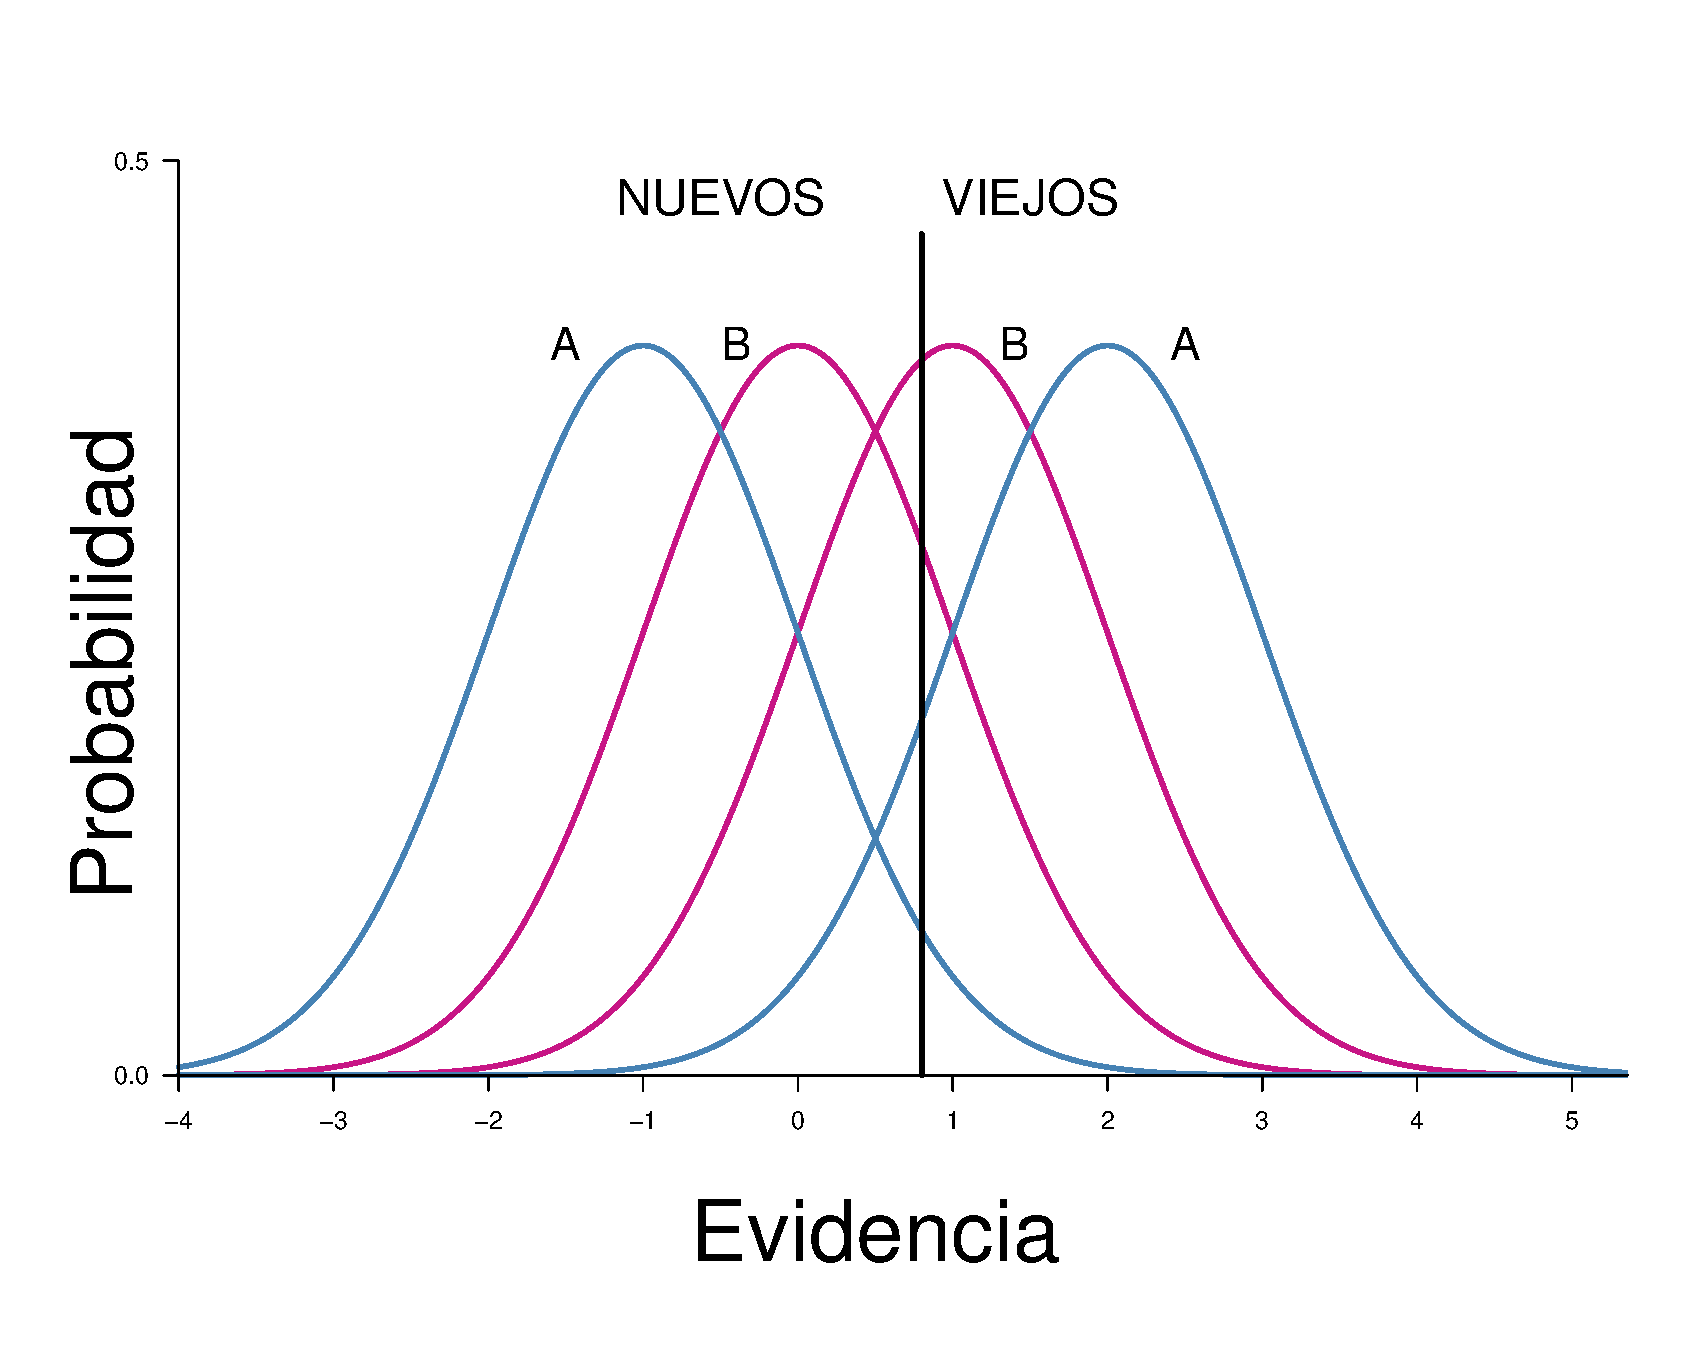
\includegraphics[width=0.6\textwidth]{Figures/EfectoEspejo_YesNo}
\decoRule
\caption[Efecto Espejo en tareas de detección binarias]{Interpretación del patrón de respuestas reportado en tareas de reconocimiento Sí/No donde se presenta más de una clase de estímulos, ($FA(A) < FA(B) < H(B) < H(A)$), asumiendo que los participantes responden con base en un sólo criterio de elección.}
\label{fig:Ejem_Espejo_YesNo}
\end{figure}

El patrón de respuestas identificado en este tipo de tareas sugiere que las cuatro distribuciones se despliegan sobre el eje de evidencia tal y como se muestra en la Figura~\ref{fig:Ejem_Espejo_YesNo}: tomando la SDT como marco de referencia, las tasas reportadas de Falsas Alarmas y Hits para las clases A y B reflejan el área de las distribuciones de ruido y señal que caen por encima del criterio. La figura presenta un ejemplo ideal, donde las distribuciones Nuevas no sólo reflejan el órden de las distribuciones Viejas, sino que también mantienen la misma distancia entre sí.\\

\item \underline{Efecto Espejo con Escalas de Confianza}\\

En estudios de memoria de reconocimiento donde se comparan los puntajes de confianza emitidos entre dos clases de estímulos A y B, se encuentra la siguiente relación:

\begin{center}
$P(NuevoA) < P(NuevoB) < P(ViejoB) < P(ViejoA)$\\
donde $P()$ es el puntaje \textbf{promedio} asignado a los estímulos Nuevos y Viejos de cada clase de estímulo, en Escalas de Confianza donde los valores más altos señalan una mayor confianza en los juicios \textit{Viejo} y los valores más bajos, en \textit{Nuevo} (Glanzer y cols., \citeyear{Glanzer1993}).\\
\end{center}

\begin{figure}[h]
\centering
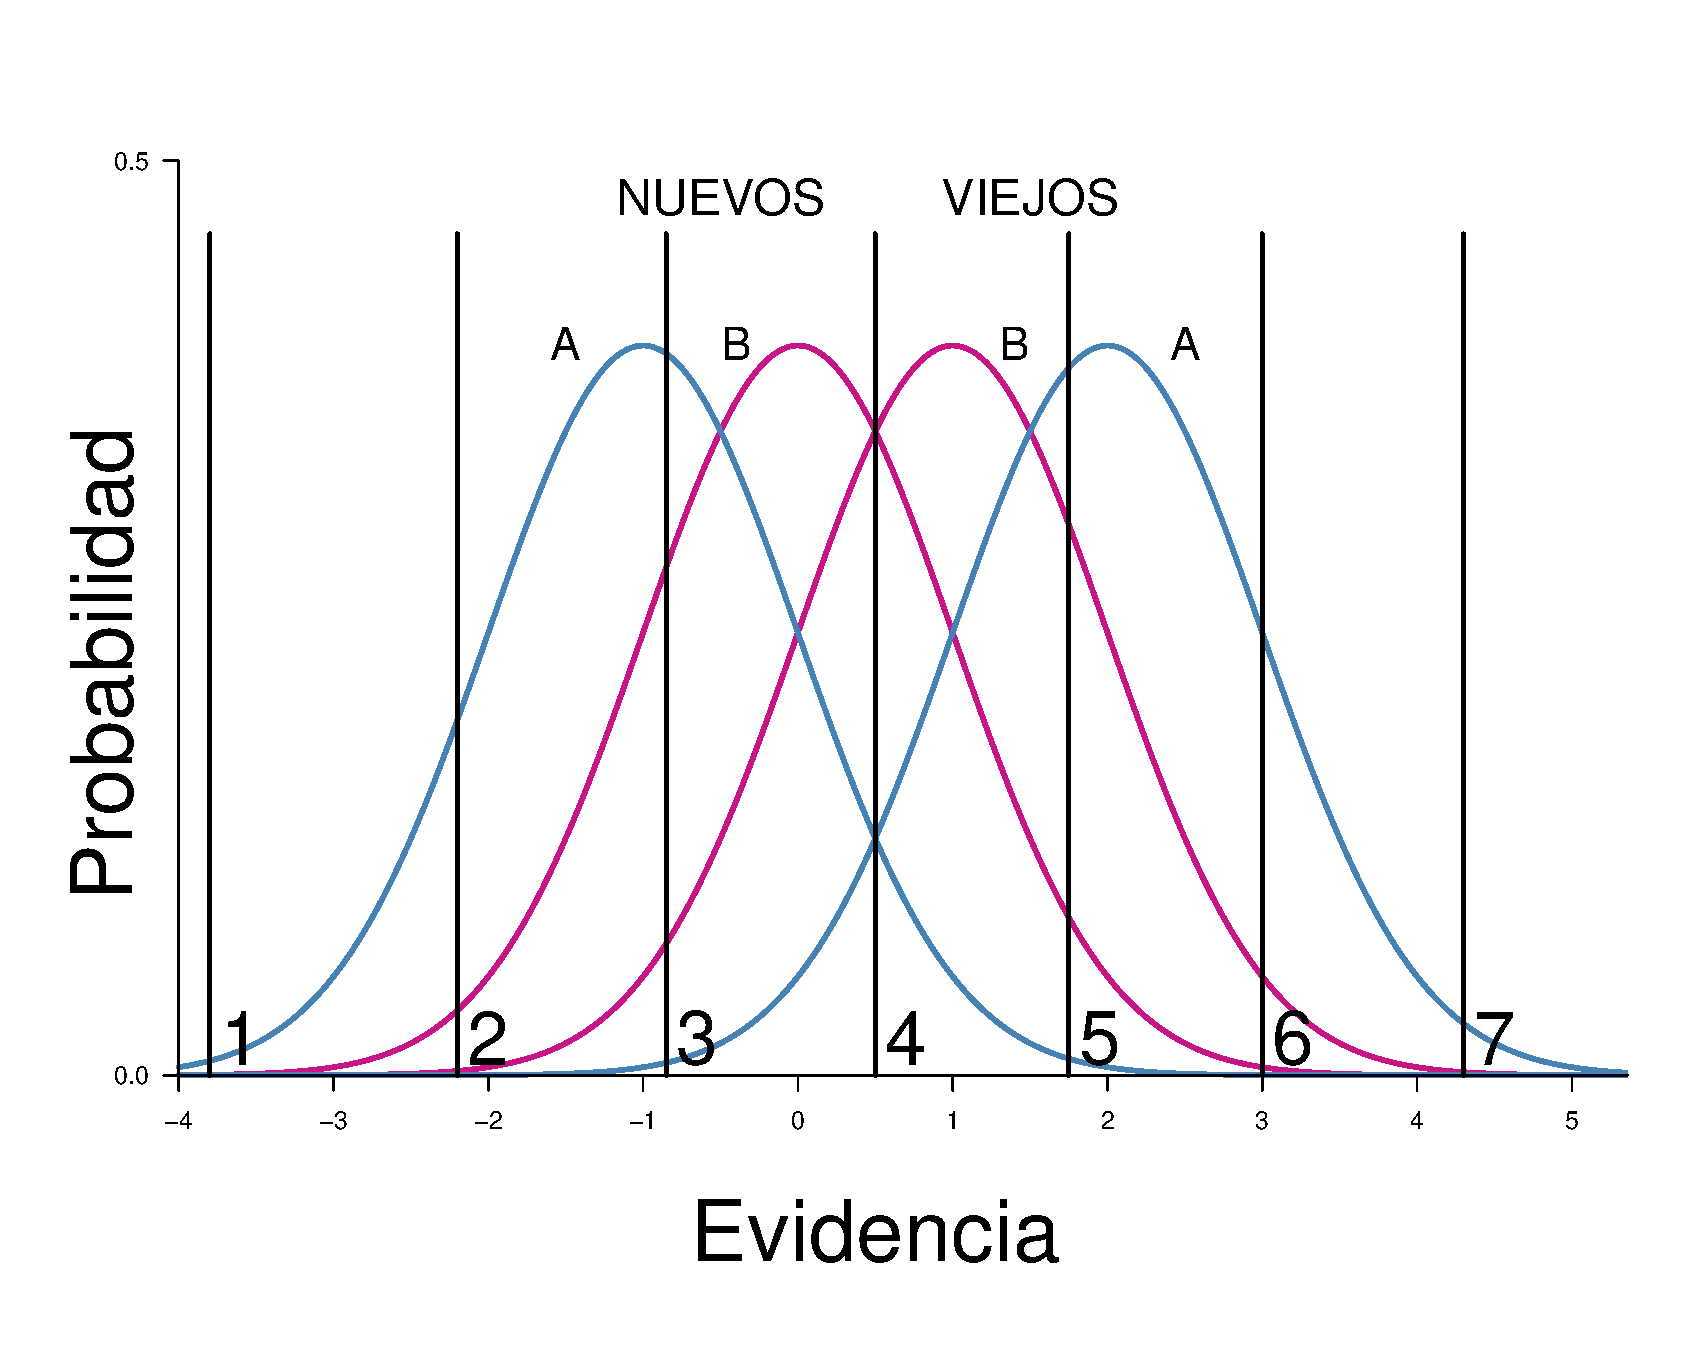
\includegraphics[width=0.6\textwidth]{Figures/EfectoEspejo_Puntajes}
\decoRule
\caption[Efecto Espejo en tareas de detección con Escala de Confianza]{Interpretación del patrón de respuestas reportado en tareas de reconocimiento con Escala de Confianza con más de una clase de estímulos ($P(NuevoA) < P(NuevoB) < P(ViejoB) < P(ViejoA)$). Asumiendo que se utilizan los mismos sub-criterios de elección para todos los ensayos, el promedio de los puntajes asignados a cada subconjunto de estímulos resulta consistente con el Efecto Espejo.}
\label{fig:Ejem_Efecto_Punt}
\end{figure}

De acuerdo con la SDT clásica (McNicol, \citeyear{McNicol2, McNicol5}), se asume que los participantes sitúan múltiples criterios de elección sobre el eje de evidencia para decidir qué puntaje de confianza emitirán para cada estímulo presentado, dependiendo cuál sea el último en ser rebasado por la \textit{familiaridad} evaluada. La Figura~\ref{fig:Ejem_Efecto_Punt} ilustra cómo esta idea y la representación del Efecto Espejo es compatible con los puntajes promedios asignados a los estímulos pertenecientes a cada una de las cuatro distribuciones. Las distribuciones de la clase A, que ocupan los valores más extremos del eje de evidencia, obtienen puntajes promedio más extremos que las distribuciones de clase B.\\

%\item \underline{Efecto Espejo en Tareas de Elección forzada entre dos alternativas}\\

%Como se mencionó previamente, en las Tareas de Elección forzada de $m$ Alternativas se presenta a los participantes en cada ensayo un número $m$ de estímulos, de los cuales $m-1$ contienen Ruido y sólamente $1$, la Señal.\\

%En el caso particular de los estudios en Memoria de Reconocimiento que proporcionan evidencia sobre la prevalencia y consistencia del Efecto Espejo, se refieren tareas de Elección Forzada de 2 alternativas. En dichos experimentos, se presenta a los participantes varias parejas conformadas por uno de los posibles estímulos con Señal ($ViejoA$ o $ViejoB$) y uno con Ruido ($NuevoA$ o $NuevoB$), siendo su tarea elegir cuál de estos dos estímulos le fue presentado durante la fase de estudio. De tal forma que en este tipo de estudios hay cuatro posibles tipos de parejas a presentar a los participantes en cada ensayo, (las \textit{parejas de comparación estándar}):\\

%\begin{itemize}
%\item Señal A VS Ruido A  (o ViejoA VS NuevoA)\\
%\item Señal A VS Ruido B (o ViejoA VS NuevoB)\\
%\item Señal B VS Ruido A (o ViejoB VS NuevoA)\\
%\item Señal B VS Ruido B (o ViejoB VS NuevoB)\\
%\end{itemize}

%En tareas de elección forzada entre 2 alternativas donde se incluyen las parejas de comparación estándar ya descritas, la evidencia a favor del Efecto Espejo se reporta a partir de las siguientes relaciones:\\

%\begin{center}
%$P(ViejoB, NuevoB) < P(ViejoB,NuevoA)$\\
%y\\
%$P(ViejoA, NuevoB) < P(ViejoA,NuevoA)$\\
%\end{center}
%\begin{center}
%donde $P$ implica la proporción de veces que el primer elemento de cada paréntesis es elegido sobre el segundo, cuando se solicita a los participantes que señalen el estímulo que se les haya presentado en la fase de estudio, \citep{Glanzer1993}.\\
%\end{center}

%Al interpretar los datos obtenidos en este tipo de tareas se asume que los participantes responden en cada ensayo eligiendo el estímulo con el valor más alto, en términos de su ubicación sobre el eje de decisión. Las parejas de comparación estándar formadas en experimentos que presentan evidencia a favor del Efecto Espejo están compuestas por un estímulo extraído de alguna de las distribuciones de estímulos Viejos y un estímulo proveniente de una distribución de estímulos Nuevos. De acuerdo con la representación gráfica de la localización de las cuatro distribuciones (ver Figura~\ref{fig:Ejem_EfectoEspejo}), existe una mayor distancia entre la distribución de estímulos Nuevos A (la distribución en el extremo izquierdo) y cualquiera de las dos distribuciones de estímulos Viejos, que entre estas y la distribución de estímulos Nuevos B (la segunda distribución de izquierda a derecha). Así, el patrón de respuestas reportado en este tipo de estudios hace sentido a la luz del orden en que se despliegan las cuatro distribuciones subyacentes: los participantes aciertan en mayor proporción -pues eligen el estímulo Viejo- en las parejas compuestas por un estímulo Nuevo A, ya que la distribución correspondiente se encuentra más alejada -y es por tanto, más discriminable- de las distribuciones de estímulos Viejos.\\

%Como un control adicional, en este tipo de experimentos se incluyen dos parejas adicionales (denominadas \textit{parejas de comparación nula}), que se componen por estímulos A y B, del mismo mismo tipo:\\

%\begin{itemize}
%\item Señal A VS Señal B (o ViejoA VS ViejoB)\\
%\item Ruido A VS Ruido B (o NuevoA VS NuevoB)\\
%\end{itemize}

%Mientras que en las elecciones observadas entre las parejas de comparación estándar se interpretan en términos de las distancias entre las distribuciones de estímulos Viejos y las distribuciones de estímulos Nuevos, las parejas de comparación nula proporcionan información acerca de la separación entre las distribuciones del mismo tipo de ensayo, pero diferente clase de estímulo. Si las respuestas de los participantes son consistentes con la representación gráfica del Efecto Espejo, se espera encontrar que:\\

%\begin{center}
%$P(ViejoA, ViejoB) > 0.5$\\
%y\\
%$P(NuevoB, NuevoA) > 0.5$\\
%\end{center}
%\begin{center}
%donde nuevamente $P$ representa la proporción de veces que se eligió el primer elemento de cada paréntesis como aquel que fue presentado anteriormente y $0.5$ señala la proporción que se esperaría encontrar si se asumiera que los participantes responden al azar, \citep{Glanzer1993}.\\ 
%\end{center}

%El punto clave detrás de la interpretación de las elecciones observadas en las parejas de comparación nula es que están compuestas por dos estímulos que representan el mismo estado -que al elegir cualquiera de estos el participante estaría cometiendo el mismo tipo de acierto o error- y, que en teoría, deberían ser elegidos por los participantes con la misma probabilidad (con proporciones cercanas al azar, $0.5$). Sin embargo, si la representación gráfica del Efecto Espejo es un reflejo apropiado de la ejecución de los participantes en este tipo de tareas, se espera encontrar una preferencia hacia la elección de los estímulos que provengan de la distribución más orientada hacia la derecha sobre el eje de evidencia. Por ejemplo, en el caso de las parejas de comparación nula compuestas por dos estímulos Nuevos A y B, se espera que los participantes elijan con una proporción superior al azar a los estímulos B, puesto que provienen de una distribución que cubre valores más altos sobre el eje de la evidencia que la distribución Nuevos A, \citep{Glanzer1993}.\\

\end{itemize}

En un inicio, los patrones de respuestas del ahora llamado Efecto Espejo fueron reportados en la literatura en memoria de reconocimiento como Efecto de Frecuencia de las Palabras (Schulman, \citeyear{Schulman1967}), ya que fueron encontrados por primera vez en estudios donde las clases entre las cuales se comparaba el desempeño de los participantes estaban compuestas por palabras \textit{poco comúnes} y palabras \textit{muy comunes}, de acuerdo a la frecuencia con que se usan (Kucera y Francis, \citeyear{Kucera1967}). Dichos estudios, realizados con diferentes protocolos experimentales (Glanzer y Bowles, \citeyear{Glanzer1976}; Bowles y Glanzer, \citeyear{Bowles1983}; Glanzer y Adams, \citeyear{Glanzer1990}), demostraron consistentemente que las palabras poco comúnes eran reconocidas con mayor precisión, tanto como Nuevas como Viejas (clase A), y que las palabras comúnes se confundían con mayor facilidad (clase B). No fue hasta que se demostró que los mismos patrones de respuesta aparecen a lo largo de una gran variedad de estudios donde las clases A y B son definidas en función a distintos factores -manipulando variables tales como la complejidad, la ortografía o la veracidad de los enunciados presentados, o bien, presentando estímulos cuyas características se sabe tienen una influencia en la precisión con que se les reconoce en presentaciones posteriores, como palabras con significado concreto (A) vs abstracto (B), imágenes (B) vs palabras (A), o rostros comúnes (B) vs rostros poco comúnes (A), entre otras (Glanzer y cols., \citeyear{Glanzer1993}; Greene, \citeyear{Greene1996}; Glanzer, Kim y Adams, \citeyear{Glanzer1998})-, que se comenzó a hablar del Efecto Espejo como una regularidad general, propia de la memoria de reconocimiento (Allen y Garton, \citeyear{Allen1968}; Glanzer y cols., \citeyear{Glanzer1993}).\\

\subsection{Relevancia, implicaciones e interpretaciones}\\

A primera vista, el patrón de respuestas identificado como Efecto Espejo podría parecer trivial: si sabemos que la principal diferencia entre las clases de estímulos presentadas en este tipo de estudios es la precisión con que sus elementos son reconocidos al presentarse más de una vez -siendo la clase A más fácil de reconocer que la clase B-, tiene sentido esperar que los participantes tengan un mejor desempeño general (más aciertos y menos errores) en la clase A. Sin embargo, al interpretar las tasas de ejecución observadas bajo el marco de la SDT, no parece claro por qué debería haber más de una distribución de ruido (como sugieren las diferencias encontradas entre las Falsas Alarmas registradas por cada clase), en tanto que en el contexto de la memoria de reconocimiento, se trata de elementos que no han sido presentados y deberían resultar igualmente \textit{familiares} -o a efectos prácticos, \textit{desconocidos}-.\\

Existen dos grandes formas en que el Efecto Espejo ha sido abordado en la literatura en memoria de reconocimiento:\\

\begin{enumerate}
\item Como reflejo de procesos cognitivos que subyacen a la ejecución de los participantes en tareas de reconocimiento (tanto en la fase de estudio, como en la fase de reconocimiento).\\

\item Como evidencia de que los modelos de memoria derivados de la SDT no describen adecuadamente el actuar de los mecanismos involucrados en la Memoria de Reconocimiento.\\
\end{enumerate}

Dentro de los modelos y teorías desarrollados para dar cuenta de lo que el Efecto Espejo podría estar sugiriendo acerca del funcionamiento de la memoria de reconocimiento se distinguen varias aproximaciones.\\

Una primera forma de interpretar el Efecto Espejo -y probablemente la más sencilla de todas- apela a las estrategias de respuesta \textit{deliberadamente} empleadas por los participantes. Este tipo de explicaciones se sustentan en el hecho de que las discrepancias entre las tasas de Falsas Alarmas desaparecen cuando se solicita explícitamente a los participantes que \textit{no adivinen} su respuesta (Greene, \citeyear{Greene1996}). Por ejemplo, la hipótesis de Distribución de las Respuestas supone que los participantes asumen por \textit{default} que la cantidad de estímulos Viejos y Nuevos a presentárseles durante el experimento es la misma y en consecuencia, modulan la cantidad de respuestas afirmativas que emiten. Este tipo de explicaciones implican también que los participantes pueden distinguir entre las dos clases de estímulos presentadas, de forma que, dado que los elementos Viejos de la clase A se identifican con mayor precisión ($Hits(A) > Hits(B)$), \textit{acumulan} una cantidad grande de respuestas afirmativas que compensan restringiendo la emisión de juicios afirmativos en los ensayos donde se les muestra estímulos de la misma clase que no contienen la Señal, reduciendo en consecuencia la tasa de Falsas Alarmas registrada para la clase A ($F.Alarmas(A) > F.Alarmas(B)$) (Greene, \citeyear{Greene1996}).\\

Un problema evidente con esta primera aproximación es que viola uno de los elementos clave detrás de la interpretación del Efecto Espejo como una fenómeno significativo y consistente en memoria de reconocimiento: el supuesto de que los participantes responden a partir de un sólo conjunto de criterios de elección que utilizan indistintamente entre los estímulos de clase A o B. En otras palabras, este tipo de explicaciones sólo permitirían dar cuenta de experimentos donde las clases A y B son fáciles de distinguir entre sí y dejan fuera el resto de los experimentos en que se ha encontrado evidencia del Efecto Espejo, sin que los participantes sepan que están siendo evaluados a traves de más de una clase de estímulos (Glanzer y cols., \citeyear{Glanzer1998}).\\

Una segunda aproximación implica asumir que las clases de estímulos empleadas en estos estudios difieren en el efecto que tienen sobre los procesos superiores involucrados en las tareas de reconocimiento. En otras palabras, este segundo conjunto de explicaciones asume que cada clase de estímulos A y B es procesada de manera distinta por los participantes. Como uno de los ejemplos más representativos de este tipo de explicaciones se encuentra la Teoría de Atención/Verosimilitud (Glanzer y cols., \citeyear{Glanzer1993}). Dicha teoría funciona como un modelo de muestreo de rasgos que se asume que todos los estímulos a presentar están compuestos por un número fijo de rasgos ($N$), de los cuales, algunos se presentan \textit{marcados} desde su primera aparición como \textit{rasgos familiares} ($p(new)$) y otros son marcados como tales una vez que se interactúa con ellos ($p(new) + [\alpha(i)* (1-p(new))]$). Esta teoría asume que la diferencia fundamental entre  las clases de estímulos probadas ($i$) es que elicitan distintos gradientes de atención que van a repercutir en el número de rasgos atendidos (\textit{muestreados}) por los participantes ($n(i)$) dentro de $N$, definiendo una \textit{tasa de marcaje} propia de cada clase ($\alpha(i)$).\\

En otras palabras, el proceso mediante el cual se explica el Efecto Espejo de acuerdo a la Teoría de Atención/Verosimilitud es el siguiente:\\

\begin{enumerate}
\item Todos los estímulos están compuestos por una cantidad $N$ de rasgos.\\

\item Todos los estímulos comienzan con una cierta proporción de rasgos marcados como \textit{conocidos}.
\begin{center}
$p(A,nuevo) = p(new)$ \qquad y \qquad $p(B,nuevo) = p(new)$\\
donde la cantidad de rasgos marcados inicialmente es la misma en las clases A y B.\\
\end{center}

\item A y B difieren en el número de rasgos que los participantes muestrean al interactuar con cada estímulo.
\begin{center}
$n(A) > n(B)$\\
La clase A es más atendida que B.\\
\end{center}

\item De acuerdo con $n(i)$, A y B tienen su propia tasa de muestreo.
\begin{center}
$\alpha(A) = \frac{n(A)}{N}$ \qquad y \qquad $\alpha(B) = \frac{n(B)}{N}$\\
donde si $n(A) > n(B)$ entonces, $\alpha(A) > \alpha(B)$\\
\end{center}

\item Al interactuar con los estímulos en la fase de estudio, los participantes muestrean cierto número de rasgos y marcan aquellos que no lo estén con anterioridad, ($\alpha(i)*(1-p(new))$).\\

\item En la fase de reconocimiento, los estímulos presentados previamente tienen una mayor proporción de rasgos marcados que los estímulos nuevos:
\begin{center}
$p(A,viejo) = p(new) + [\alpha(A)*(1-p(new))]$\\
y \quad $p(B,viejo) = p (new) + [\alpha(B)*(1-p(new))]$\\
\end{center}
\end{enumerate}

De acuerdo con la Teoría de Atención/Verosimilitud, los participantes registran sus respuestas en la fase de reconocimiento con base en la cantidad de rasgos \textit{marcados} muestreado ($x$). La probabilidad de observar cierto valor de $x$ se describe en función a una distribución binomial con probabilidad $p(i,j)$ (donde $i$ es la clase A o B y $j$ es el tipo de estímulo: nuevo o viejos), para el total de observaciones $n(i)$ registradas en función a la clase del estímulo. Es decir:

\begin{center}
$p(x|p(i,j),n(i))$\\
\end{center}

Al observar una cantidad $x$ de rasgos marcados, los participantes emiten el juicio de reconocimiento que corresponda a dicha evidencia con mayor probabilidad, computando una razón de verosimilitudes (Glanzer y cols., \citeyear{Glanzer1993}; Hintzman, \citeyear{Hintzman1994}; Glanzer, Hilford y Maloney, \citeyear{Glanzer2009}; Hilford, Maloney, Glanzer y Kim, \citeyear{Hilford2015}). De acuerdo con esta teoría, el Efecto Espejo se explica por medio de la siguiente relación:

\begin{center}
$p(x|p(A,nuevo),n(A)) < p(x|p(B,nuevo),n(B)) < p(x|p(B,viejo),n(B)) < p(x|p(A,viejo),n(A))$\\
\end{center}

En la Teoría de Atención/Verosimilitud el elemento clave para explicar las diferencias en el desempeño de los participantes entre A y B es la atención elicitada por cada clase, y el número de rasgos muestreados en consecuencia ($n(i)$). Esto resuelve el problema de las discrepancias entre las tasas de Falsas Alarmas de la siguiente forma: aunque A y B contienen el mismo número de rasgos marcados en su primera presentación ($p(A,nuevo) = p(B,nuevo)$), el número de elementos muestreados es mayor en la condición A ($n(A) > n(B)$) y por tanto, hay una mayor probabilidad de extraer rasgos marcados ($p(x|p(A,nuevo),n(A)) < p(x|p(B,nuevo),n(B))$).\\

Pese al conjunto de experimentos desarrollados para probar la solidez de la Teoría de Atención/Verosimilitud mediante la manipulación de distintas variables experimentales que deberian tener un impacto sobre los parámetros del modelo (por ejemplo, restringiendo el tiempo de estudio y/o de respuesta para modificar $n(i)$ en cada fase) y evaluando la precisión con que el modelo predice y explica los datos encontrados (Glanzer y cols., \citeyear{Glanzer1993}; Kim y Glanzer, \citeyear{Kim1993}; Glanzer, Adams e Iverson, \citeyear{Glanzer1991}), la Teoría de Atención/Verosimilitud ha sido fuertemente criticada en relación a dos grandes factores: 1) la teoría está compuesta por parámetros y supuestos innecesariamente complejos que le restan validez ecológica y 2) la teoría asume que los participantes tienen acceso a información completa sobre la estructura de la tarea y son capaces de utilizarla para realizar cómputos altamente demandantes (Hintzman, \citeyear{Hintzman1994}; Murdock, \citeyear{Murdock1998}; DeCarlo, \citeyear{DeCarlo2007}).\\

Una tercera forma de interpretar el Efecto Espejo es de manera consistente con la aplicación de la SDT al análisis de las tareas de reconocimiento: asumiendo que los participantes registran sus respuestas en función a la evidencia que evalúan en cada ensayo (\textit{la fuerza de memoria} o \textit{familiaridad} contenida en el eje de evidencia), sin necesidad de recurrir a ningún tipo de cómputo adicional (Hintzman, \citeyear{Hintzman1994}). Bajo esta perspectiva, la única diferencia que existe entre las clases A y B -sin importar si pueda justificarse el por qué de ella- es la \textit{fuerza de memoria} que contienen, o bien qué tan familiares resultan para los participantes. Por ejemplo, en los estudios donde se usan distintos niveles de \textit{Palabras frecuentes} para delimitar las clases de estímulos a comparar, las palabras poco comúnes parecen ser más fáciles de recordar y reconocer (A) y las palabras comúnes parecen confundirse con mayor facilidad (B). De acuerdo a este tipo de explicaciones, las palabras comúnes Nuevas (B,Nuevo) tienen un mayor grado de familiaridad que los estímulos Nuevos poco comúnes (A,Nuevo), por lo que la separación de las dos distribuciones de estímulos Nuevos tiene sentido. A su vez, dado que las palabras poco comúnes son más salientes, se asume que se les presta más atención y terminan adquiriendo un mayor nivel de familiaridad cuando se les presenta por segunda vez que las palabras comúnes, lo que termina explicando el orden en que se presentan las distribuciones de estímulos Viejos (Glanzer y cols., \citeyear{Glanzer1993}).\\

En una dirección distinta, se encuentran las interpretaciones del Efecto Espejo que tienden a tomarle como evidencia para desacreditar el uso de la SDT para estudiar del fenómeno de la memoria de reconocimiento. Por ejemplo, un primer conflicto evidente en la interpretación del Efecto Espejo es que no siempre parece claro por qué una de las clases de estímulos a probar debería resultar \textit{más familiar} (A) que la otra (B) desde que se presenta en la fase de estudio. Aún cuando este tipo de explicaciones se sostiene de manera intuitiva para entender los resultados encontrados en estudios donde A y B se componen de palabras poco comúnes y comúnes, cuando se intenta añadir una tercer clase C, compuesta por palabras \textit{raras}, los resultados encontrados no son consistentes con lo que la interpretación del Efecto Espejo sugeriría (Rao y Proctor, \citeyear{Rao1984}; Wixted, \citeyear{Wixted1992}). En general, se esperaría que la nueva clase C añadiera dos distribuciones más sobre el eje de evidencia, que se agregarían hacia los extremos inferior y superior del mismo. Sin embargo, este no parece ser el caso.\\

Por último, se encuentran los trabajos orientados al desarrollo y evaluación de distintos modelos de detección de señales que difieren en la naturaleza que se asume tienen las distribuciones subyacentes a la tarea. Por ejemplo, asumiendo distintos tipos de distribuciones (Glanzer y cols., \citeyear{Glanzer1993}, \citeyear{Glanzer2009}) o bien, fomentando el abordaje del problema desde la perspectiva de los modelos de mezclas en detección de señales (DeCarlo, \citeyear{DeCarlo2002} ,\citeyear{DeCarlo2007}).\\

\section{Planteamiento del problema}

Como se describió en la sección anterior, el Efecto Espejo es un fenómeno empírico reportado en estudios de memoria de reconocimiento desarrollados bajo el marco de la SDT. Su consistencia a lo largo de diversos procedimientos y variables impulsó el desarrollo de distintos tipos de interpretaciones, tanto en términos de lo que podría sugerir sobre cómo opera la memoria de reconocimiento, como de la evaluación del uso del modelo de detección de señales como marco para describir la ejecución de los participantes en este tipo de tareas.\\

En contraste con la amplia variedad de propuestas desarrolladas para dar cuenta del Efecto Espejo como un fenómeno intrínseco a la Memoria de Reconocimiento, es importante señalar que dicho fenómeno no ha sido estudiado ni reportado en ningún otro tipo de tareas de detección.\\

Evaluar la generalizabilidad del Efecto Espejo a otras áreas de aplicación de la SDT se considera importante en tanto que 1) provería un contexto más amplio para interpretar el Efecto Espejo como una regularidad derivada de los supuestos establecidos por la SDT y no como un fenómeno particular de la memoria de reconocimiento y los procesos cognitivos involucrados, y 2) permitiría evaluar la pertinencia de la aplicación del modelo de detección de señales para interpretar los resultados obtenidos en este tipo de tareas en memoria de reconocimiento.\\

El trabajo de tesis aquí presentado no se preocupa en evaluar de forma alguna las propuestas teóricas y formales desarrolladas para dar cuenta del Efecto Espejo como un fenómeno inherente a la memoria de reconocimiento. El objetivo del trabajo de investigación realizado es meramente el de explorar la existencia de los patrones de respuesta identificados como Efecto Espejo en una tarea de detección ajena al marco de la memoria de reconocimiento. Para ello, se propuso trabajar con una tarea de detección perceptual que emula las condiciones básicas de las tareas de reconocimiento donde dicho fenómeno ha sido reportado, construyéndose las clases de estímulos A y B a partir de la revisión de la literatura en ilusiones ópticas para garantizar que estas difirieran en su discriminabilidad ($d'$).